%%%%%%%%%%%%%%%%%%%%%%%%%%%%%%%%%%%%%%%%%
% Journal Article
% LaTeX Template
% Version 1.4 (15/5/16)
%
% This template has been downloaded from:
% http://www.LaTeXTemplates.com
%
% Original author:
% Frits Wenneker (http://www.howtotex.com) with extensive modifications by
% Vel (vel@LaTeXTemplates.com)
%
% License:
% CC BY-NC-SA 3.0 (http://creativecommons.org/licenses/by-nc-sa/3.0/)
%
% Template modified by Alison Sheltong for STAT 626 Final Project.
%%%%%%%%%%%%%%%%%%%%%%%%%%%%%%%%%%%%%%%%%

%----------------------------------------------------------------------------------------
%	PACKAGES AND OTHER DOCUMENT CONFIGURATIONS
%----------------------------------------------------------------------------------------

\documentclass[twoside,twocolumn]{article}

\usepackage[greek,english]{babel} % Language hyphenation and typographical rules
\usepackage{graphicx}
\usepackage{float, enumitem}
\usepackage{amssymb,amsfonts,textcomp}
\usepackage{caption}
\usepackage{lmodern}
\usepackage{booktabs} % Horizontal rules in tables

\usepackage{hyperref} % For hyperlinks in the PDF

\usepackage{blindtext} % Package to generate dummy text throughout this template - helpful for double checking spaccing.

\usepackage[utf8x]{inputenc} %Because I like this one better than the one in the template
\usepackage{natbib}
\bibliographystyle{apalike}


\usepackage[margin=.75 in, hmarginratio=1:1,top=32mm,columnsep=20pt]{geometry} % Document margins, provided extra space for us with smaller margins than the default.

\usepackage{enumitem} % Customized lists
\setlist[itemize]{noitemsep} % Make itemize lists more compact

\usepackage{abstract} % Allows abstract customization - The italics for example.
\renewcommand{\abstractnamefont}{\normalfont\bfseries} % Set the "Abstract" text to bold
\renewcommand{\abstracttextfont}{\normalfont\small\itshape} % Set the abstract itself to small italic text

\usepackage{fancyhdr} % Headers and footers
\pagestyle{fancy} % All pages have headers and footers
\lhead{\bfseries Group 4}
\chead{\bfseries STAT 626: Time Series Analysis}
\rhead{\bfseries US Unemployment Trends} 
\lfoot{}
\cfoot{\thepage}
\rfoot{} 


\usepackage{titling} % Customizing the title section 

%----------------------------------------------------------------------------------------
%	TITLE SECTION
%----------------------------------------------------------------------------------------
\setlength{\droptitle}{-4\baselineskip} % Move the title up

\pretitle{\begin{center}\huge\bfseries} % Article title formatting
\posttitle{\end{center}} % Article title closing formatting
\title{US Unemployment Trends} % Article title
\author{%
\textsc{Joseph Blubaugh}\thanks{Plots, Data Prep, Code Management} \\[1ex] % Your name
\normalsize Statistics\\ % Your institution
%\normalsize \href{mailto:john@smith.com}{john@smith.com} % Your email address
\and % Uncomment if 2 authors are required, duplicate these 4 lines if more
\textsc{Sean Roberson}\thanks{Presentor} \\[1ex] % Second author's name
\normalsize Mathematics, Industrial\\ % Second author's institution
\and 
\textsc{Akarshan Puri}\thanks{Model selection and fitting} \\[1ex] 
\normalsize Electrical Engineering\\ 
\and 
\textsc{Alison Shelton}\thanks{Write-up} \\[1ex] 
\normalsize Statistics\\ 
\and 
\textsc{Travis Lilley}\thanks{Diagnostics} \\[1ex] 
\normalsize Statistics\\ 
\and
\textsc{Bo Pang}\thanks{Model fitting and plots} \\[1 ex]
\normalsize Psychology, Statistics
\vspace*{.5 cm}
}
%\institute[Texas A\&M] % I'm not sure yet how to add this in with the way that I put in the author names.
	%	{Texas A\&M \newline College Station, Texas}
\date{July 25, 2016 \vspace*{.25 cm}} % Final write-up due date plus a bit of extra space
\renewcommand{\maketitlehookd}{%
\begin{abstract}
\noindent The information from above is from the original presentation.  The links as to who did what should be modified probably at the end.  This is just a starting point. Also the abstract should be written last so I thought it was a good place to put this information.

\vspace*{.25 cm}
\noindent The writeup below has dummy text so I could set up the sections. I also moved some of the older write-up text to this document to start it all up.
\end{abstract}
}



%----------------------------------------------------------------------------------------

\begin{document}

% Print the title
\maketitle

%----------------------------------------------------------------------------------------
%	ARTICLE CONTENTS
%----------------------------------------------------------------------------------------

%Text requiring further explanation\footnote{Example footnote}. I don't think we need footnotes


\section{Introduction}
		Unemployment has been a topic of concern throughout the United States in recent years.  The Great Recession iof 2007 was accompanied the worst unemployment crises seen since the 1930s \citep{wanberg2012individual}.   The results have been enduring, in 2010 the US job deficit was estimated to be over 10 million \citep{katz2010}. Graduate and Undergraduate college students alike are concerned over their employment prospects, wondering if their degrees will be enough to gain them a job after graduation.  These worries are well-founded as full-reovery of college graduate employment rates and earning is expected to be a slow process \cite{carnevale2015hard}.  In these times of economic uncertainty, obtaining an income generating position is not the guarantee it has seemed to be in generations past.
		
Unemployment has far-reaching consequences that extends beyond financial security. Unemployment is linked to psychological difficulties, including depression and suicide, and even physical deterioration \citep{wanberg2012individual, insecure, suicide}. A study of Greek students found a relationship between parental unemployment and PTSD symptoms related to bullying \citep{kanellopoulos2014epa}. In Nigeria, unemployment has been linked to insurgency and terrorism \citep{terrorism}. Given the impact that unemployment has on fiscal, mental, and physical health, reasearch into unemployment patterns an important part of developing policies to improve the welfare of the local, national, and global populace.

\subsection{Goal}
		The purpose of our project is to examine trends in unemployment in the United States. We will focus on the years surrounding the Great Recession of 2007, 1992 to 2015.  Our goal is to forcast unemployment into 2016. 

\subsection{Data}

The unemployment data being examined was obtained from the seasonaly adjusted, monthly, Civilian Unemployment Rate Series (UNRATE), published by the Bureau of Labor Statistics (BLS).  This series includes unemployment figures from January of 1948 to  May of 2016 \citep{blsrefsa}.  The response variable being analyzed is the unemployment rate defined as the percentage of the labor force that is unemployed.  In defining this variable, the BLS restricts this to, ``people 16 years of age and older, who currently reside in 1 of the 50 states or the District of Columbia, who do not reside in institutions (e.g., penal and mental facilities, homes for the aged), and who are not on active duty in the Armed Forces''.

Resession dates were obtained from the National Bureau of Economic Research (NBER) \citep{NBER2016}. The NBER identifies recessions and US business cycles based upon a variety of economic indicators. These include Gross Domestic Product (GDP), Gross Domestic Income (GDI), and a variety of less well known indicators such as Aggregate hours of work in the total economy.

We also explored several potential predictor variables that are potentially related to unemployment.  Industrial Production measures enterprise output of the U.S. establishments \citep{BGFS2016}. Value of Manufacturers' New Orders for All Manufacturing Industries refers to manufacturer's sales and inventory, except for New Orders from the Semicondutor Industry \citep{vmno}. The Purchase Only House Price Index for the United States follows sales for a specific set of single-family homes \citep{fhfa2016}. We also included Retailers Sales \citep{retail2016} and Total Construction Spending \citep{construction2016}.



%------------------------------------------------

\section{Exploratory Analysis}
		\begin{figure}[H]
		\centering
		\caption{Plot of the original data}
		\label{fig:unemployment}
		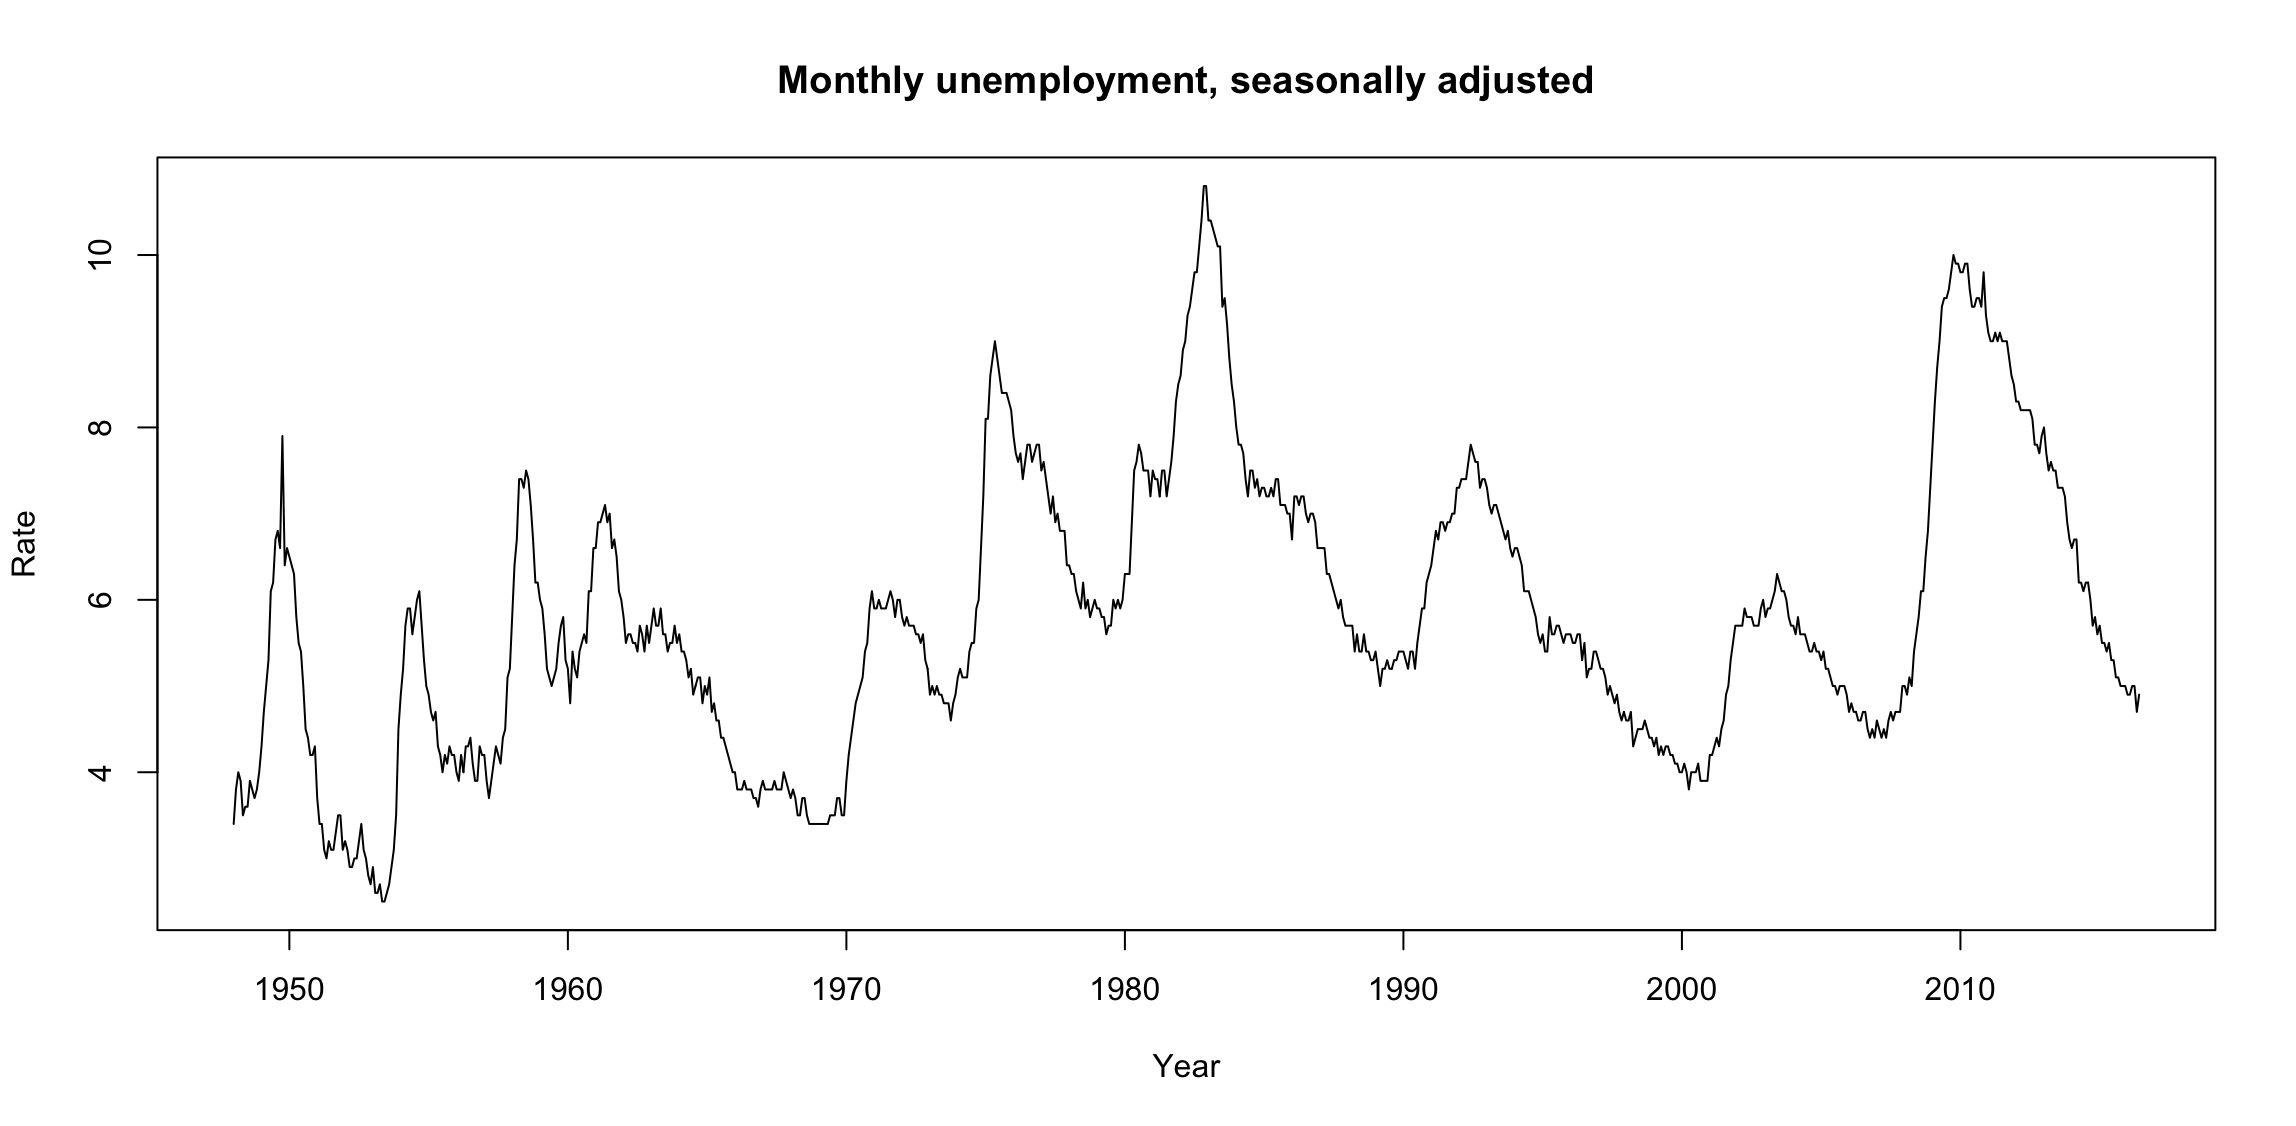
\includegraphics[width=\linewidth]{images/unemployment_total_sa}
	\end{figure}
	
			\begin{figure}[H]
		\centering
		\caption{Smoothed unemployment for the study time period}
		\label{fig:presunemp}
		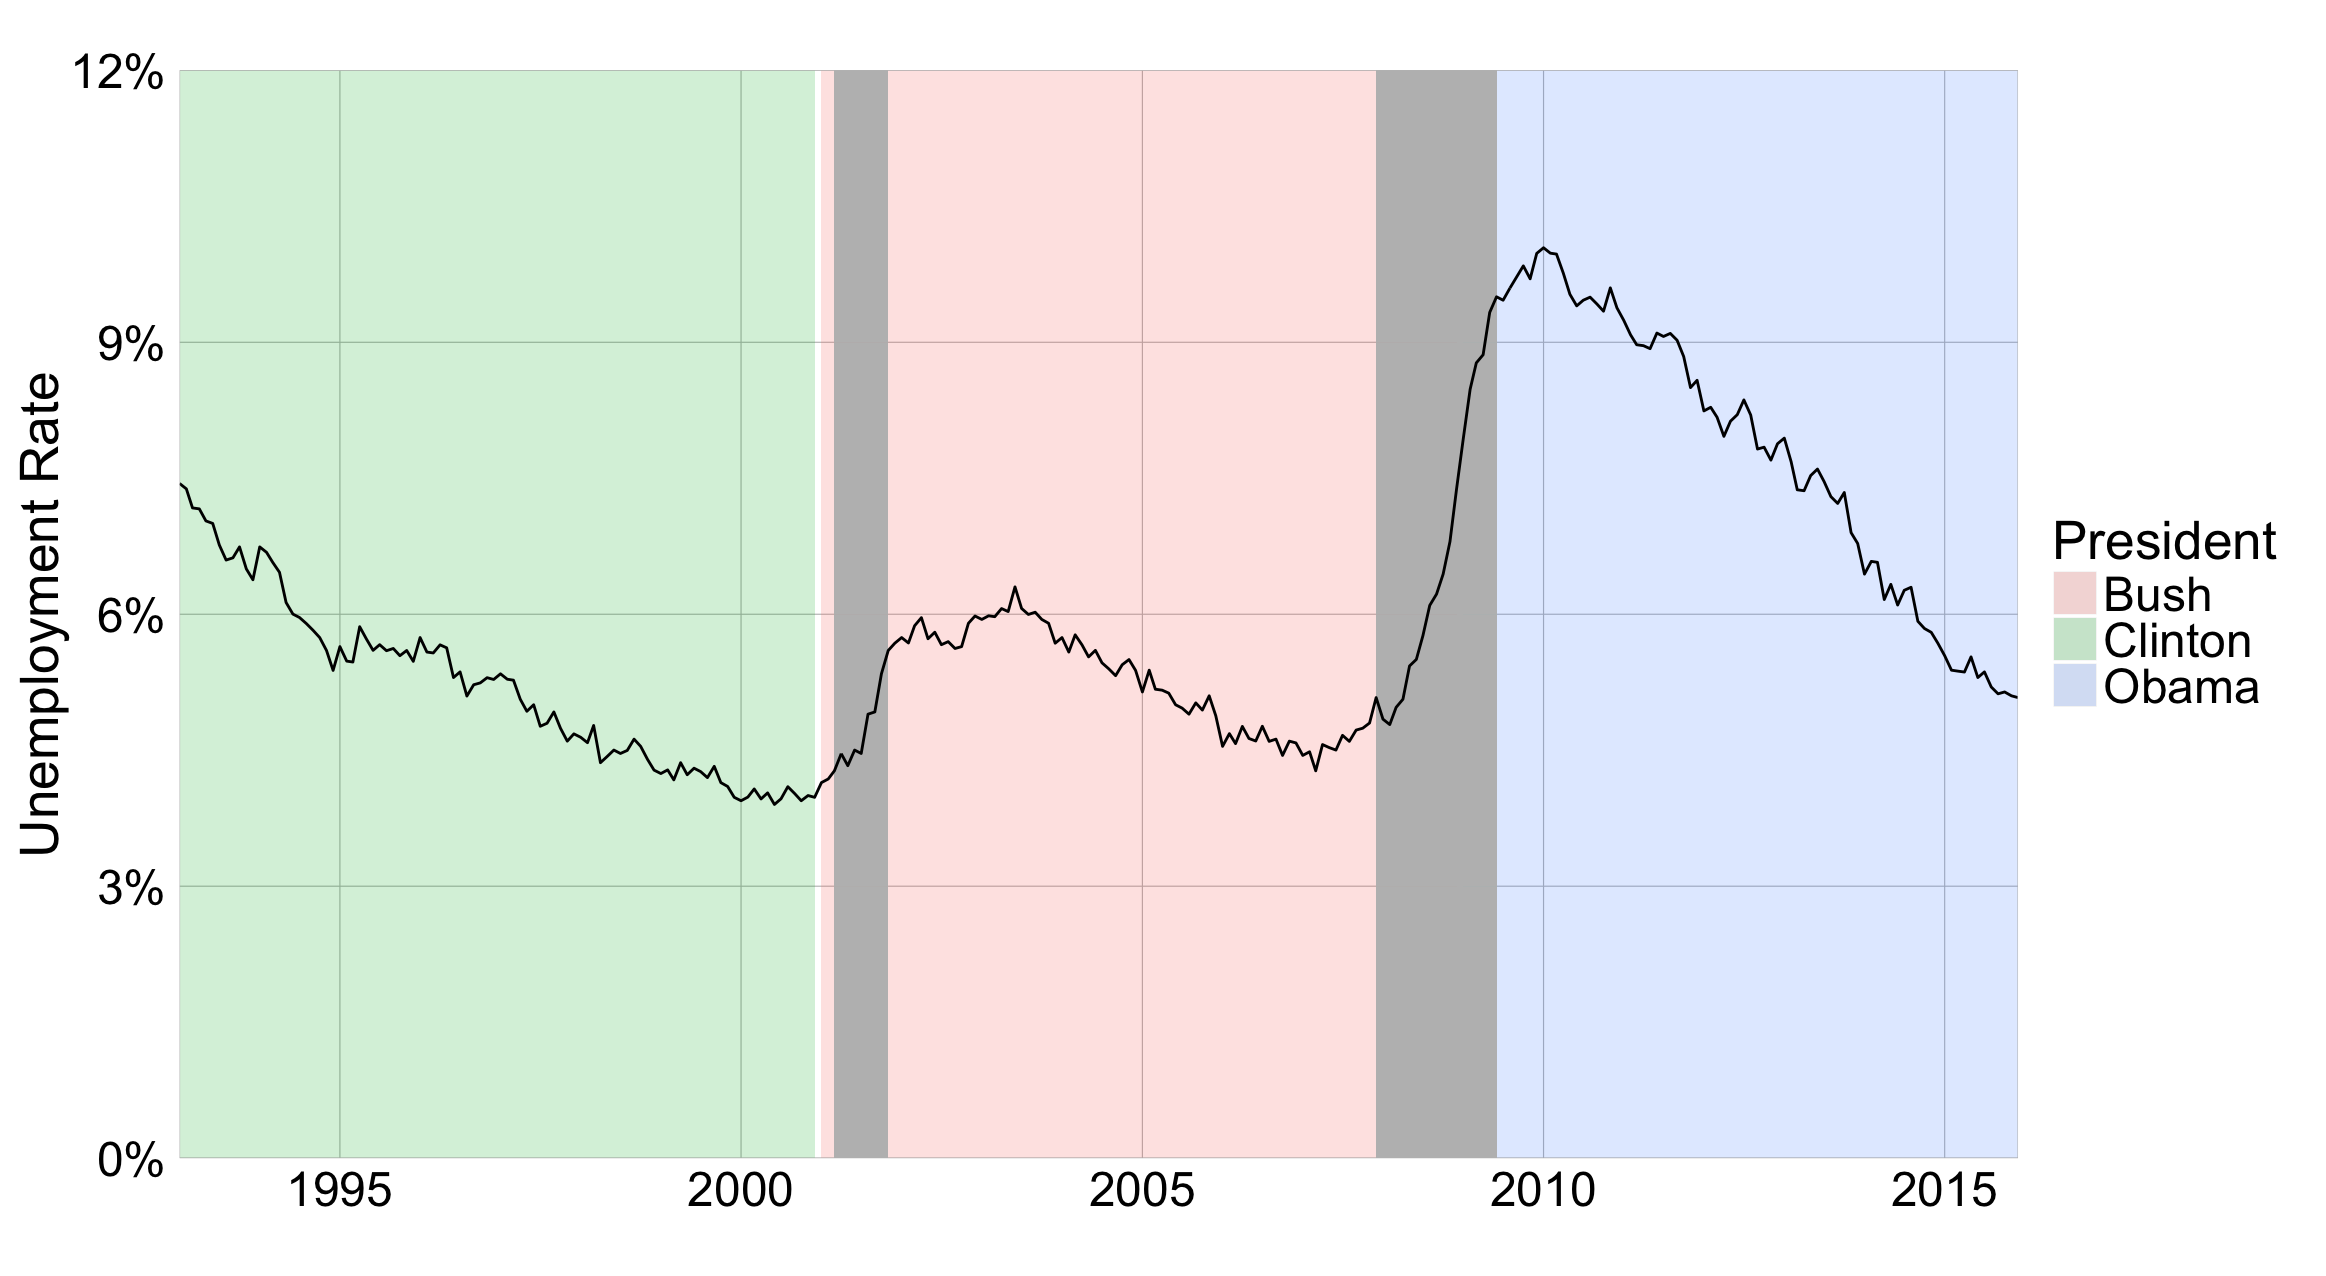
\includegraphics[width=\linewidth]{images/presunemp}
	\end{figure}


As a first step, the data was plotted over time to identify any obvious patterns visually, considering the seasonlly adjusted version of the unemployment rate, see Figure \ref{fig:unemployment}.  Overall, unemployment appears relatively volatile.  There are several time periods of sudden spikes in the unemployment rate, followed by a slower recovery period. This countercyclical movement is consistent with the descriptions of unemployment data found in the literature \citep{katz2010, Montgomery1998, shimer2012reassessing}. 

Due to marked potential differences in the trend surrounding times of economic downturn, such as those that occured after World War II and in the 70s and the 80s, we have chosen to limit our analysis on a more recent set of unemployment data. Ultimately, we decided to focus the time preceeding and following the Great Recession of 2007. We limited our inital analysis to 1992 to 2015, which encompases the presidential terms of Bill Clinton, George W. Bush, and Barack Obama, each serving eight years in office.  Initial graphs of the data seem to indicate that, in general, unemployment spiked at the begining of each president's term and fell gradually over the time he was in office, see Figure \ref{fig:presunemp}. There are also two noticeable spikes the represent that recessions of 2001 and 2008, respectively.  The 2008 recession also follows the burst of a housing market bubble.  These are all explanatory variables that can potentially inform unemployment patterns. A scatterplot of these predictors can be seen in Figure \ref{fig:pred_scatt}.

			\begin{figure}[H]
		\centering
		\caption{Scatterplot of unemployment and potential predictors}
		\label{fig:pred_scatt}
		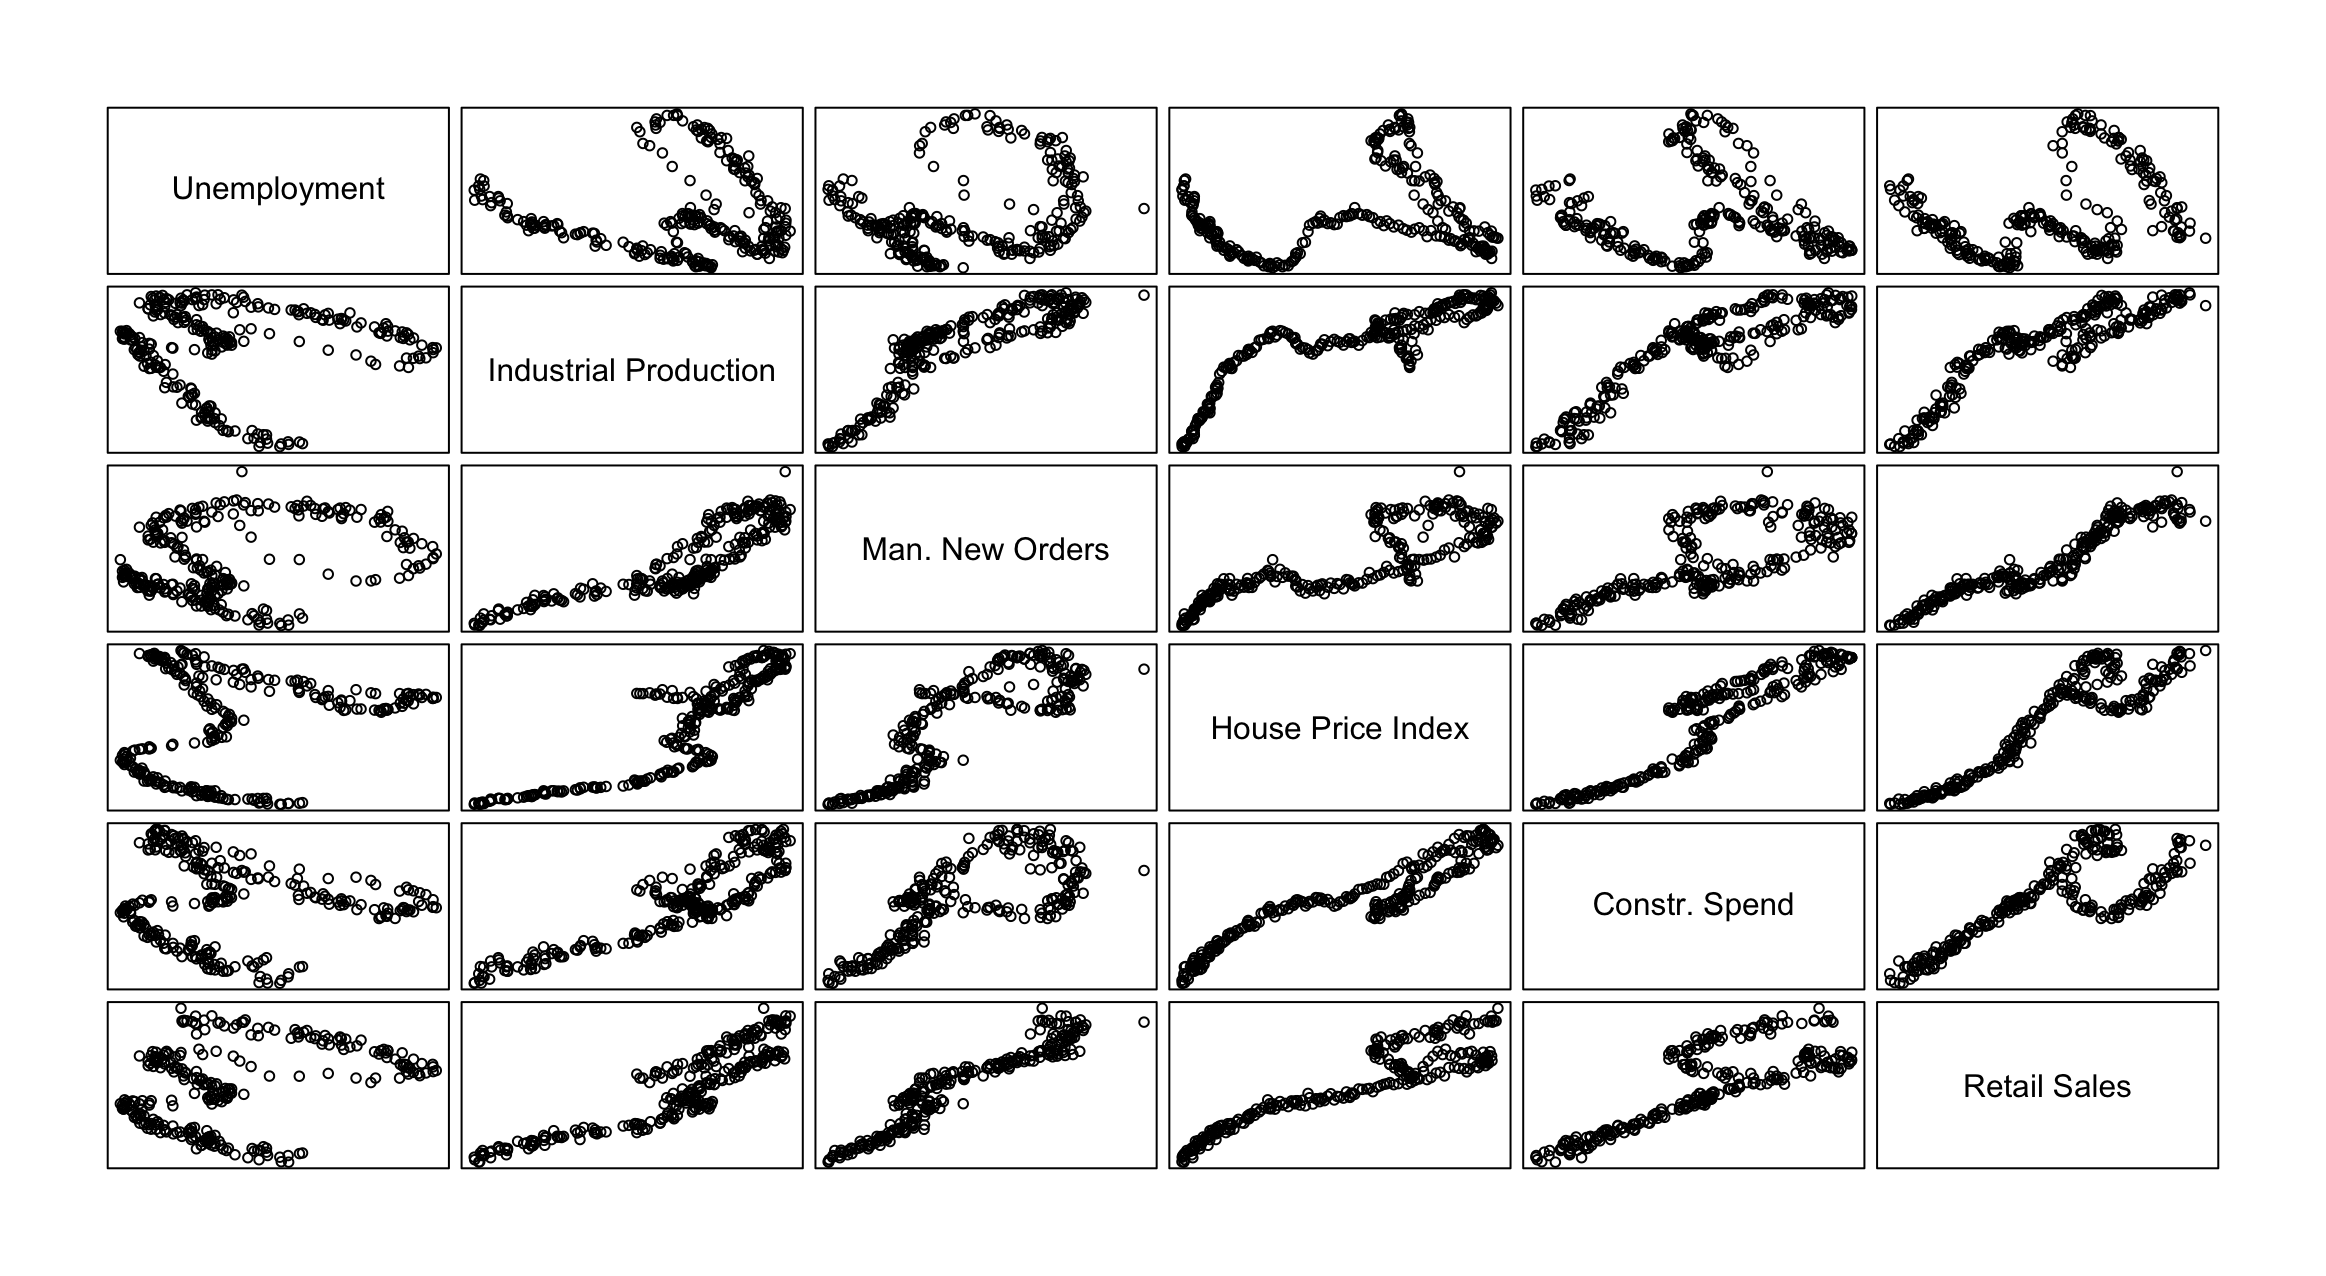
\includegraphics[width=\linewidth]{images/pred_scatt}
	\end{figure}
	

%------------------------------------------------

\section{Achieving Stationarity}

In analyzing the inital plots, it appears that the series could benefit from detrending. A graph of various potential lagged values for unemployment can be seen in Figure \ref{fig:laggedunemployment}. The high values of the correlation coffecients, particularly through lag 6 further suggest a high degree of autocorrelation within the unemployment dataset.    An Augmented Dickey-Fuller (ADF) test for stationarity was conducted to verify the nonstationarity of the unemployment data.  The ADF test tests the null hypothesis that the time series data has a unit root against the alternative that the data are stationary \citep{Shumway2006}. The Dickey-Fuller test statistic for the unemployment data is -2.1377, with a lag order of 6, and a p-value of 0.518. The high p-values suggest that we do not have a stationary model with just the raw unemployment data.
			
						\begin{figure}[H]
		\centering
		\caption{Autocorrelation of unemployment data}
		\label{fig:laggedunemployment}
		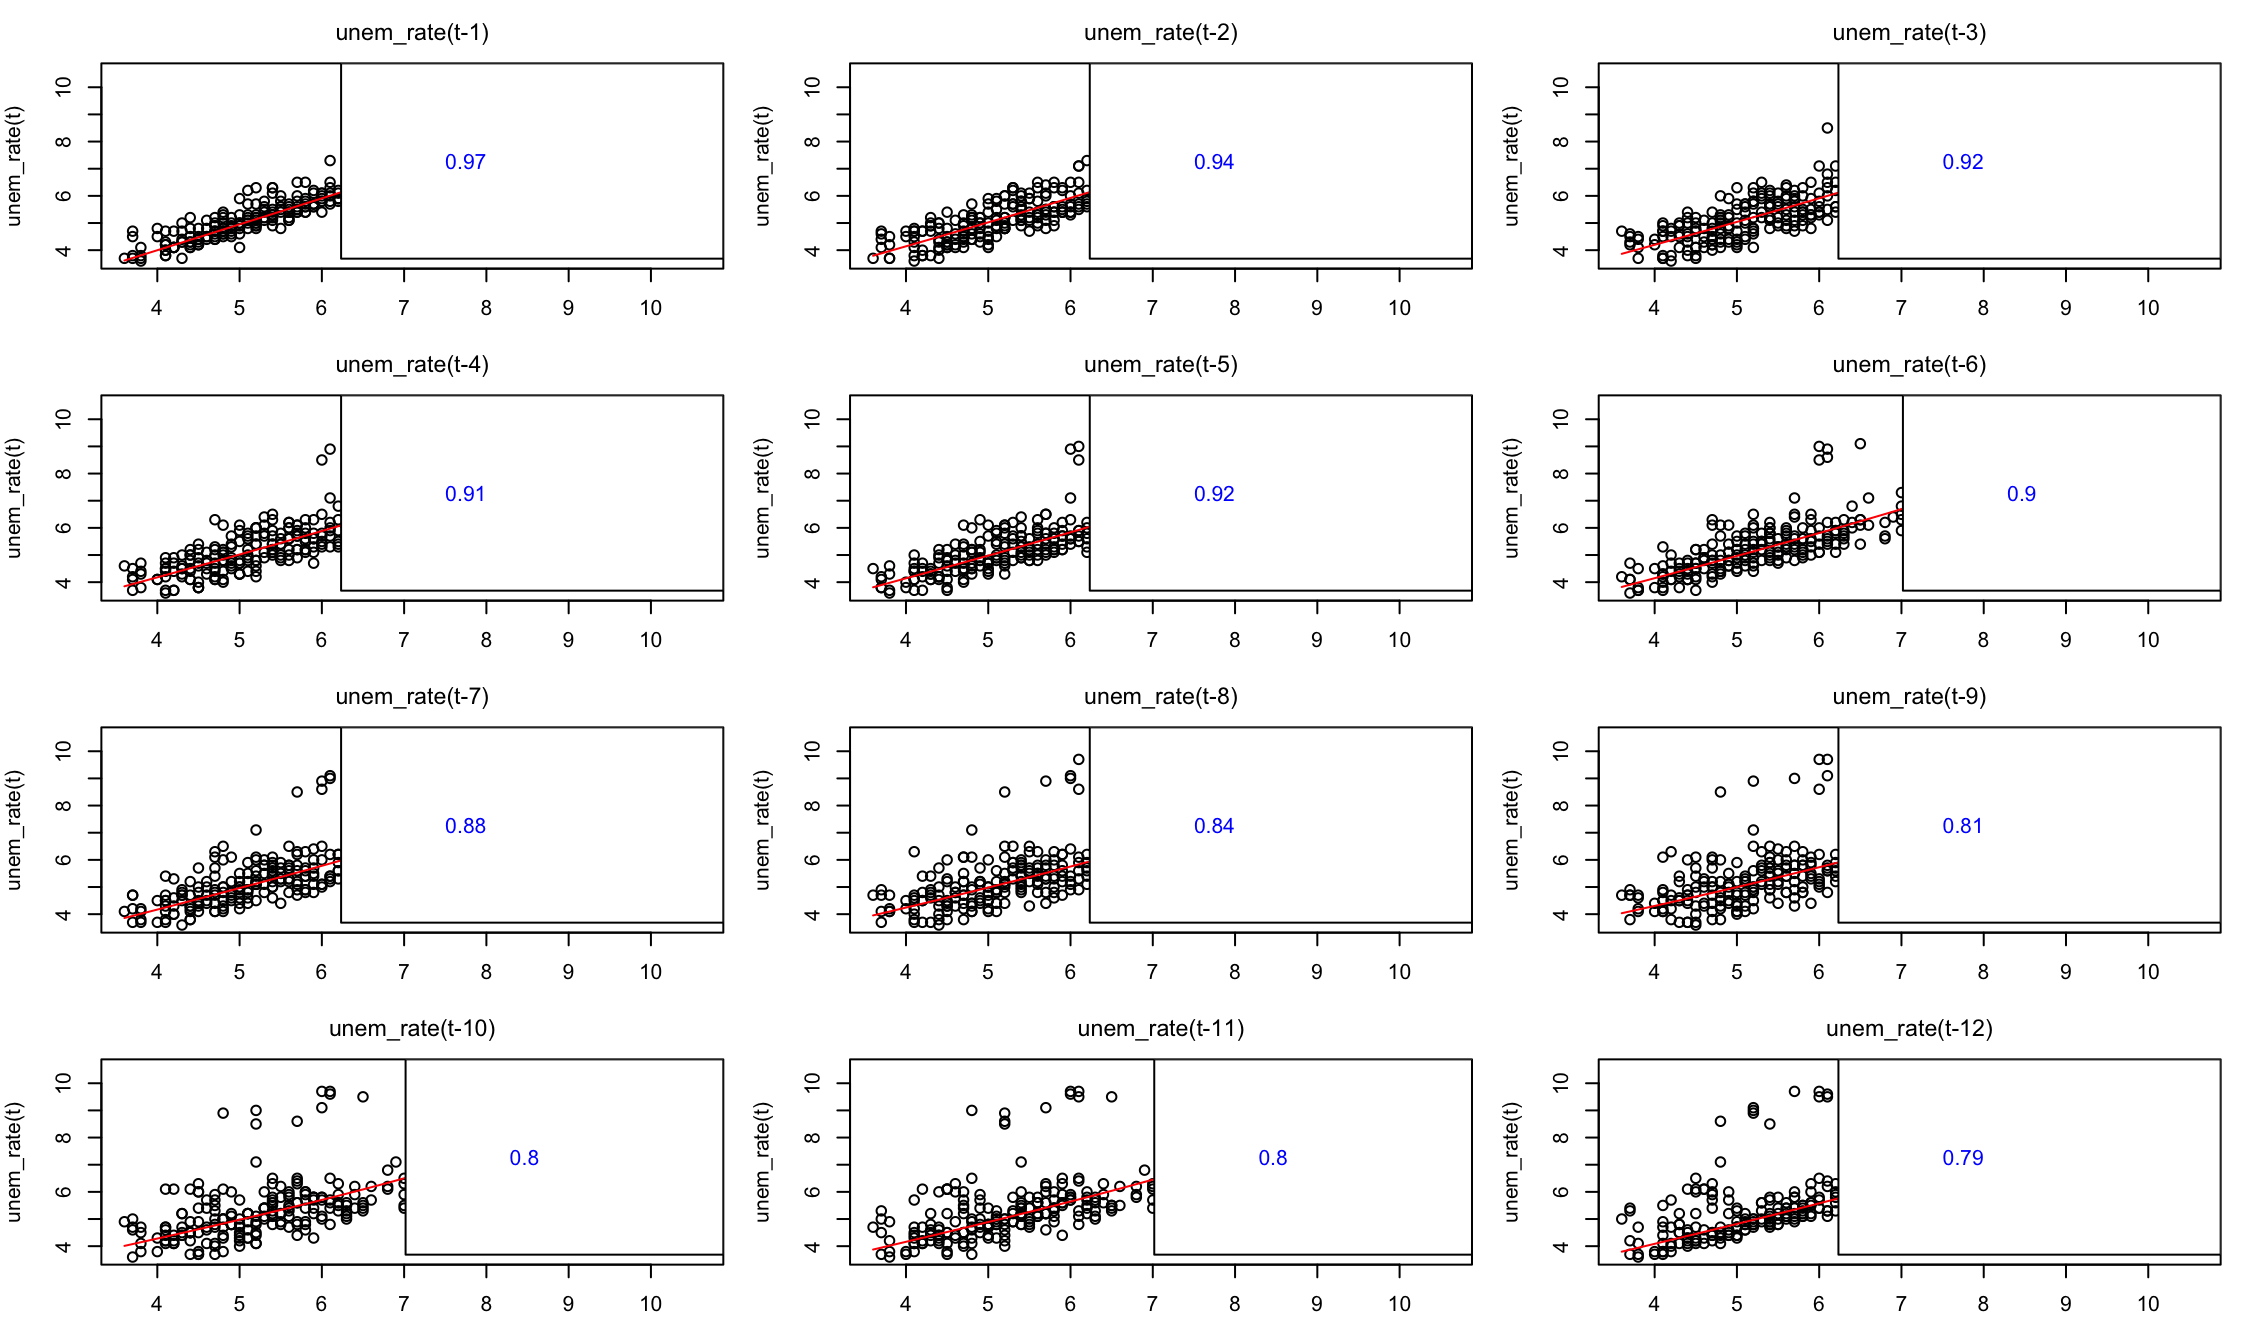
\includegraphics[width=\linewidth]{images/laggedunemployment}
	\end{figure}
			


					\begin{figure}[H]
		\centering
		\caption{Timeplots with and without differencing}
		\label{fig:seasonalunem}
		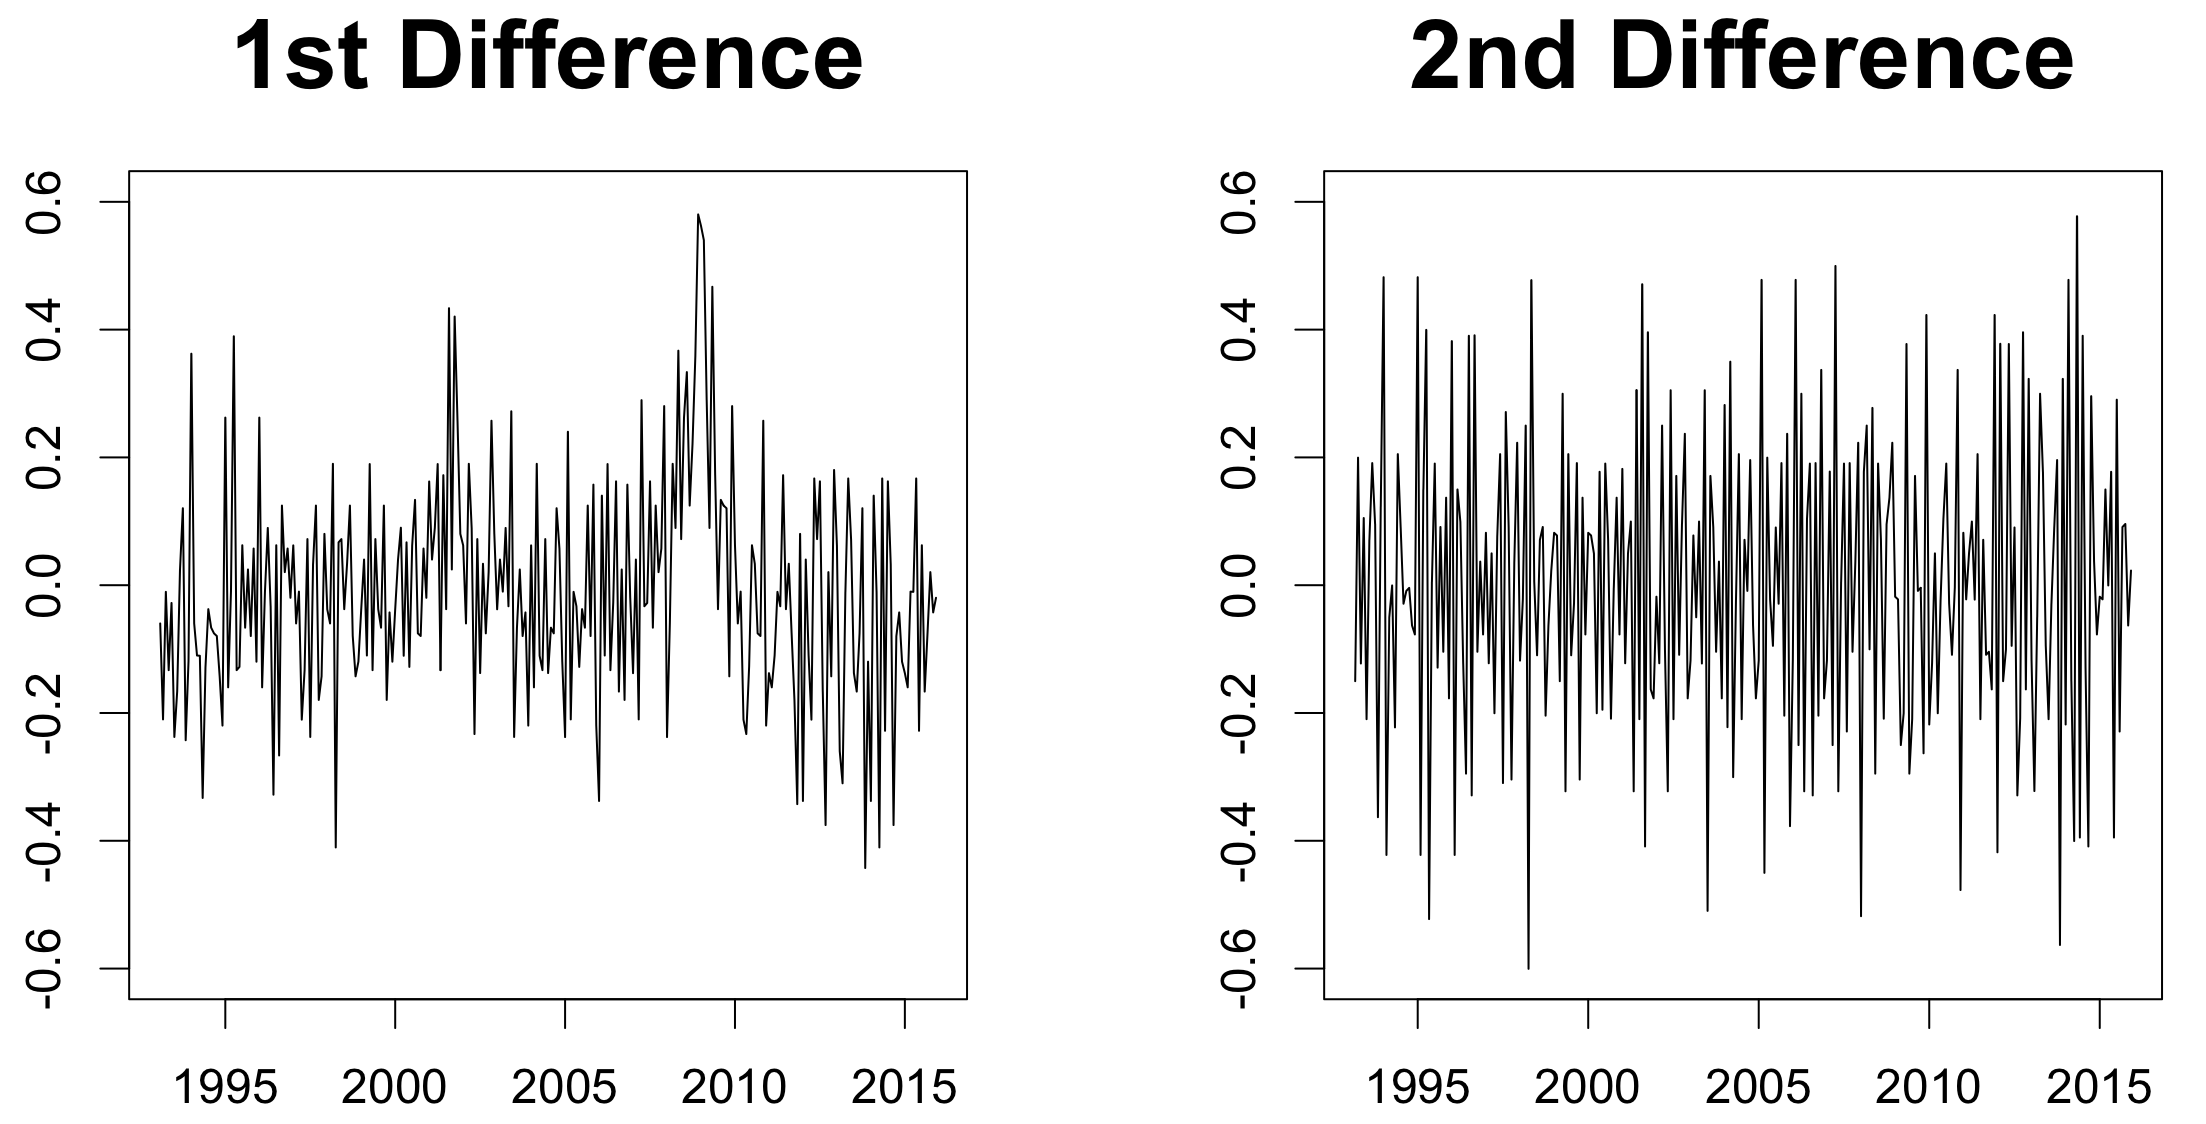
\includegraphics[width=\linewidth]{images/seasonalunem}
	\end{figure}

The first, second, and third differences of the unemployment data were plotted for seasonally adjusted unemployment data, see Figure \ref{fig:seasonalunem}. All three sets of differencing, bring the data closer to stationarity with a consistent mean and more constant variance. The associated ADF test results are given in Table \ref{tab:ADF}. Based on the p-values, there is significant evidence of stationarity with each of the differenced models. Visually, the second differences best approximate a white noise series. Futhermore, even though the ADF statistic is more negative for the \(3^{rd}\) differences there appears to be more variability in the model that includes third differences.  Therefore, the consensus in the group was to continue the model building process using second differences.

	 \begin{table}[H]
		 \centering
		 \caption{ADF Test Results}
		 \label{tab:ADF}
		 \begin{tabular}{lllll}
		 \hline
		 \textbf{Model} & \textbf{Statistic} & \textbf{Lag order} & \textbf{p-value}\\ \hline
		  1\(^{st}\) difference &  -9.3595 & 6 &\( < 0.01\)\\
		  2\(^{nd}\) difference &  -9.3595 & 6 & \( < 0.01\)\\			  
		  3\(^{rd}\) difference &  -13.02 & 6 & \( < 0.01\)\\		 \hline
		 \end{tabular}
		 \end{table}

  


%------------------------------------------------

\section{Model Building}
  
  We began our model building process by inspecting the correlogram (ACF plot) and partial correlogram (PACF plot) of tthe unemployment data, see Figure \ref{fig:acfpacf}. The ACF seems to tail off and the PACF seems to cut off at either 1 or 3.  A tailing ACF function with a PACF that cuts off at \(p\) suggests an AR(\(p\)) model \citep{Box2008}. Therefore, these inital plots suggest a possible AR(1) or AR(3) model. When looking at the ACF and PACF of the second differences, we have evidence of a possible mixture model with \(d=2\). For example, an ACF of difference \(d\) that decays exponentially after lag 1 with a PACF that is dominated by an exponential decay pattern after lag 1 would be evidence of an ARIMA(1,\(d\),1) model . Therefore, it is worthwhile considering ARIMA models such as ARIMA(1,2,1). Of course predictor variables may help to improve the predictive strength of our models, therefore models with regressors and Vector Autogressive Models (VAR) were considered as well.
  
    \begin{figure}[H]
    	\centering
     	\caption{ACF \& PACF Plots}
     	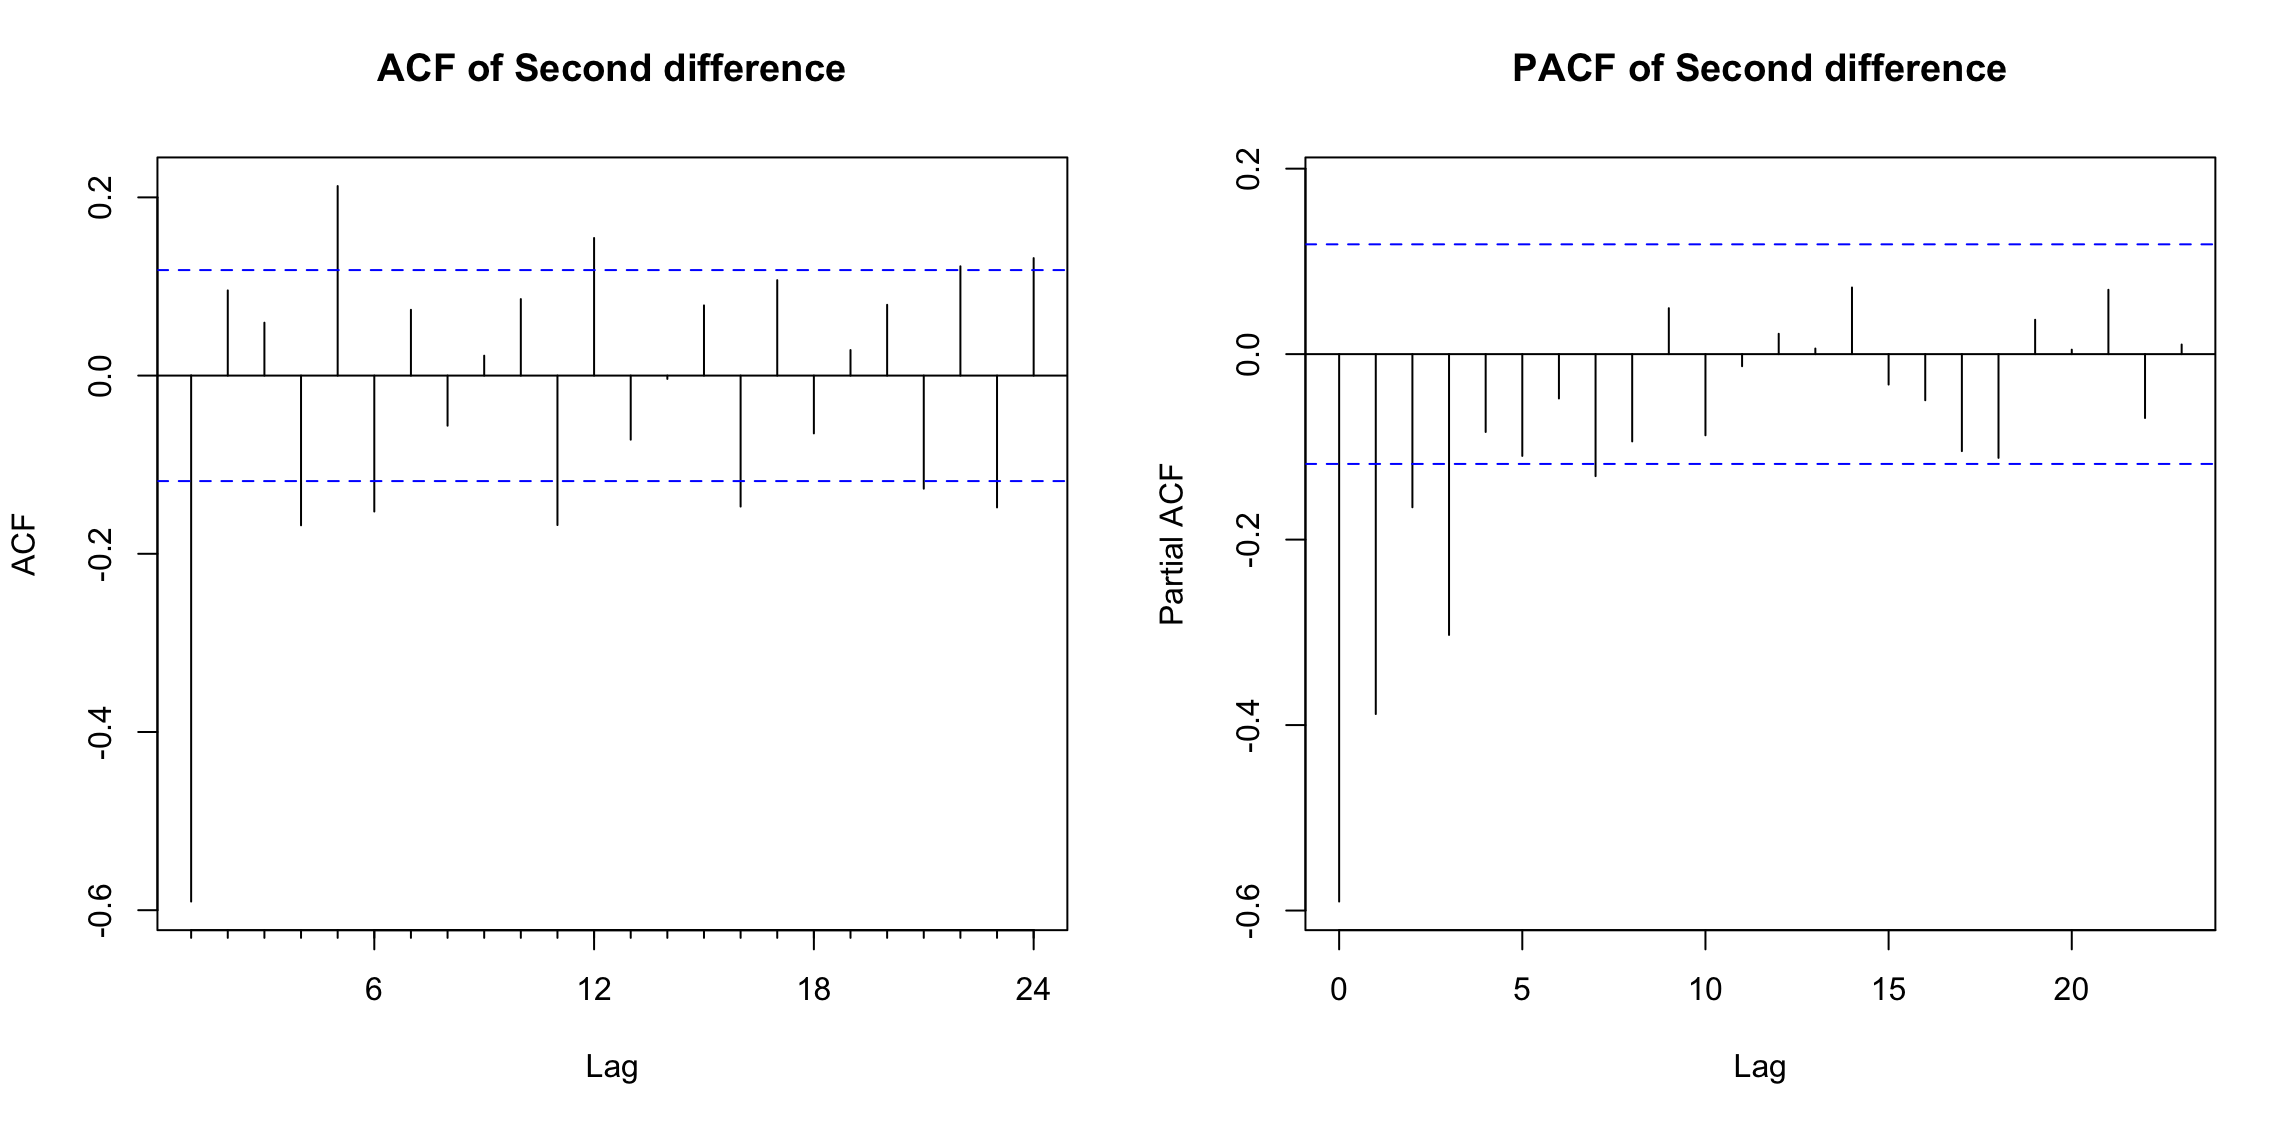
\includegraphics[width=\linewidth]{images/acfpacf}
     	\label{fig:acfpacf}
     	\caption{ACF \& PACF Plots of Second Differences}
     	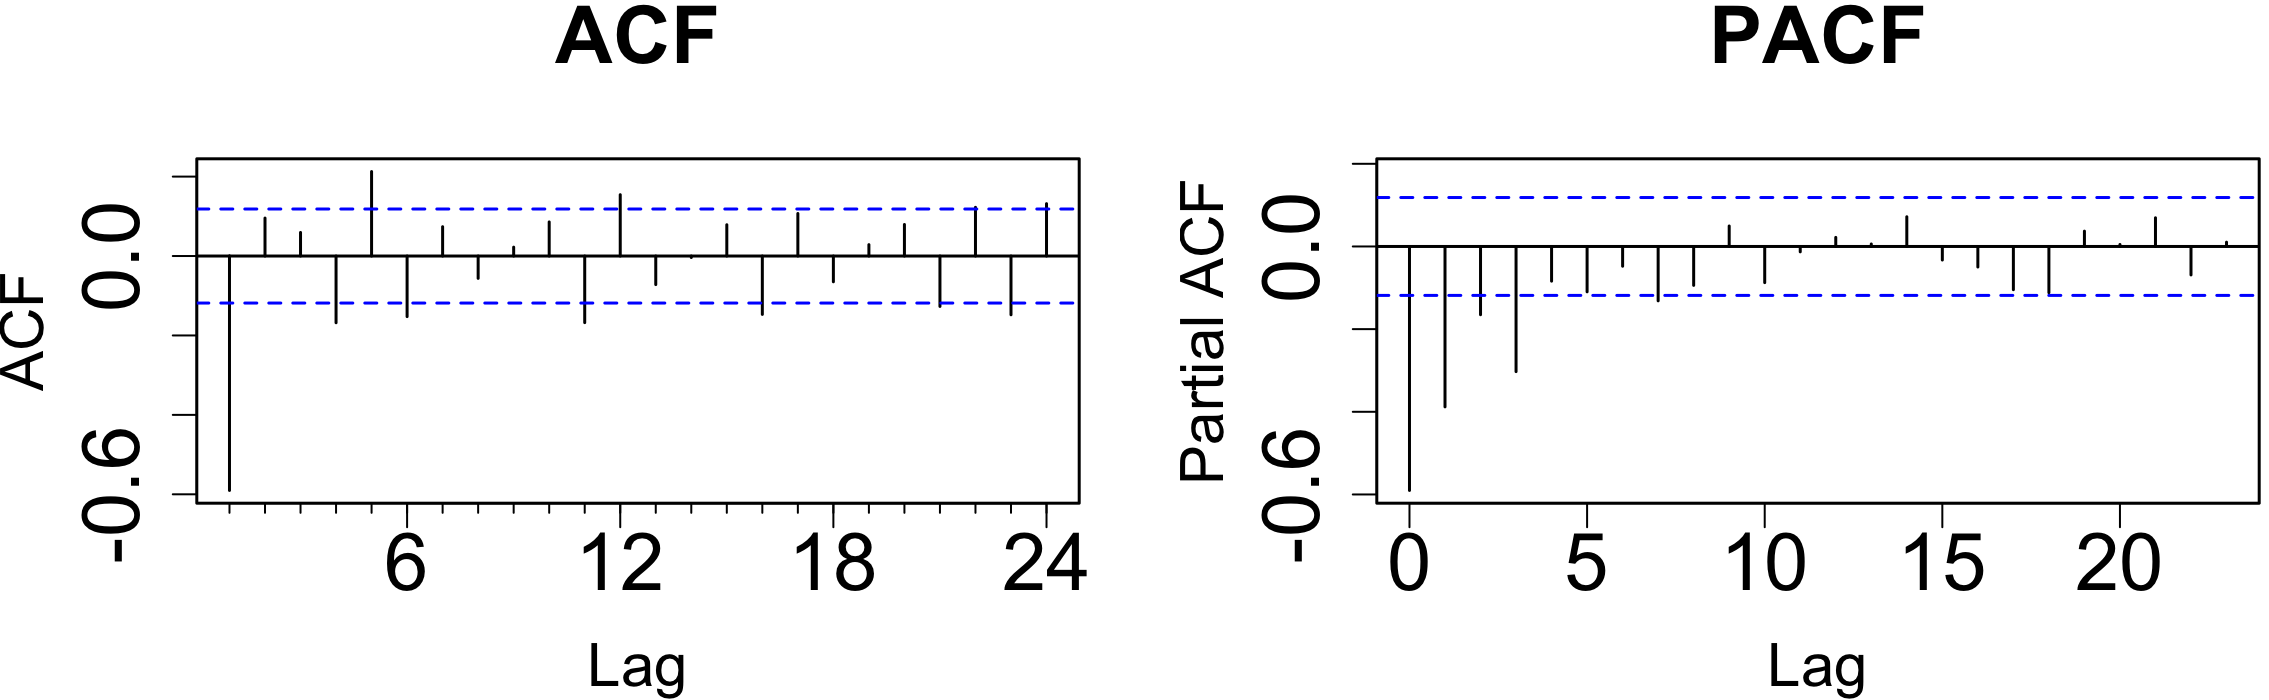
\includegraphics[width=\linewidth]{images/acfpacf2d}
     	\label{fig:acfpacf2}
      \end{figure}


\subsection{Models Considered}

\subsubsection{ARIMA Models}

Given the potenial of ARIMA models to represent the unemployment data we began by exploring three potential models without regressors, ARIMA(1,2,1), ARIMA(2,2,2), and ARIMA(3,2,3). Although model 3, ARIMA(3,2,3), has the lowest AIC of the three models, model 1, the ARIMA(1,2,1) model, has the lowest BIC. Model 1 is also the most parsimonious model of the three. So of the three intitial models, without regressors, we chose to retain model 1.  

    \begin{figure}[H]
    	\centering
     	\caption{ARIMA(1,2,1) residual diagonostics.}
     	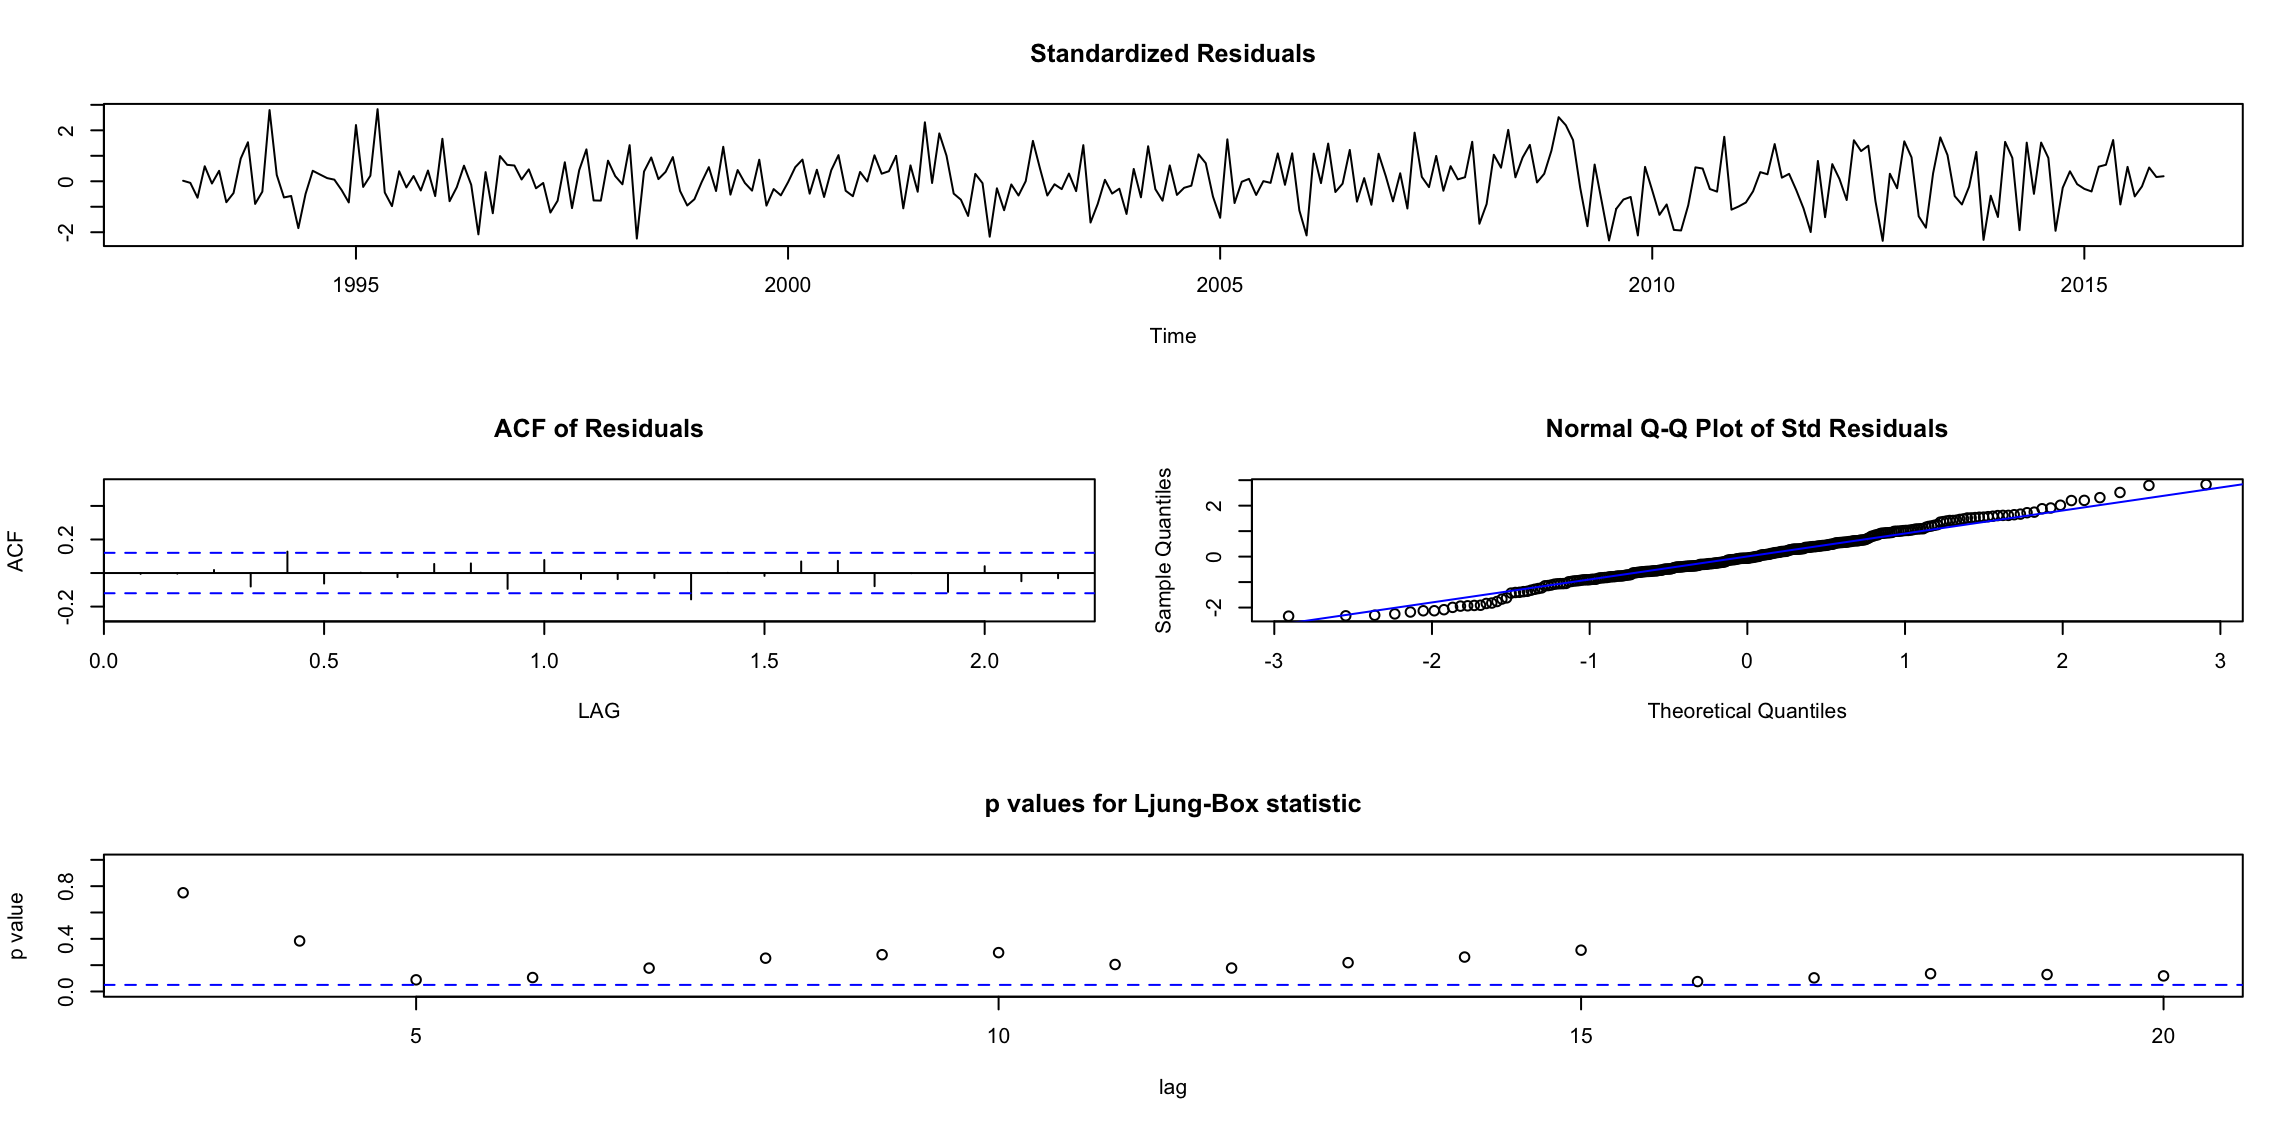
\includegraphics[width=\linewidth]{images/sarima1}
     	\label{fig:sarimamod1}
     \end{figure}


Figure \ref{fig:sarimamod1} provides the residual diagnostics for model 1. The timeplot of the standardized residuals resembles a white noise series and largely stays within two standard deviations from the expected mean of 0.  The ACF of residuals does not deviate significantly from 0, although there is a potential spike at lag 24. The normal Q-Q plot is relatively straight giving no indication that the residuals are not normally distributed. The pvalues for the Ljung-Box statistic are all relatively large, giving no indication of autocorrelation in the residuals.  Overall, model 1 seems to represent the unemployment series well.


% latex table generated in R 3.3.1 by xtable 1.8-2 package
% Sun Jul 24 08:35:48 2016
\begin{table}[ht]
\centering
\begin{tabular}{cllrrl}
  \hline
 Model & Order & Reg  & AIC & BIC & Best \\ 
  \hline
1 & 1,2,1 &  NA &   -212.30 & -201.46 & BIC \\ 
  2  & 2,2,2 & NA   & -211.81 & -193.74 &  \\ 
  3  & 3,2,3 &  NA  & -215.48 & -190.19 &  \\ 
  4  & 1,2,1 & X  & -211.56 & -182.65 &  \\ 
  5  & 2,2,2 & X   & -209.83 & -177.32 &  \\ 
  6  & 3,2,3 & X   & -215.10 & -171.74 &  \\ 
  7  & 1,2,1 &  LagX & -222.45 & -193.69 & AIC \\ 
  8  & 2,2,2 &  LagX & -220.70 & -188.35 &  \\ 
  9  & 3,2,3 &  LagX & -217.89 & -174.76 &  \\ 
   \hline
\end{tabular}
\end{table}



\begin{verbatim}
model1 <- sarima(unem, p = 0, d = 2, 
q = 1, P = 1, D = 1, Q = 0, S = 12)
model2 <- sarima(unem, p = 0, d = 2, 
q = 1, P = 3, D = 1, Q = 0, S = 12)
model3 <- sarima(unem, p = 4, d = 2, 
q = 1, P = 3, D = 1, Q = 0, S = 12)

model1$AIC; model1$BIC
[1] -2.283108
[1] -3.244063

model2$AIC; model2$BIC
[1] -2.444084
[1] -3.379008

model3$AIC; model3$BIC
[1] -2.44496
[1] -3.327824
\end{verbatim}



The Q-statistic or Ljung-Box statistic
Models 1 and 2 have similar results. Model 1 seems to perform better at the first few lags, but Model 2 does better after lag 15. Model 3 clearly perform better than the two models on the Q-statistic. Since the Model 3 is based on a reasoning our professor does not like, we may not present this model. However it at least informs us that some models based on the thought that both the ACF and PACF cuts off at certain lags might model our data better. I am not quite sure how to handle this situation. Any thoughts on this would be highly appreciated!

While going through a bunch of models, the following model seems most appropriate as noted by everyone. sarima(econ[,2],0,2,1,1,1,0,12) with the following diagnostics: [image: Inline image 2] The adf test also suggests stationarity as follows: [image: Inline image 3] Also, I am working on other predictor variables to develop a preliminary regression model.

Regarding the expectations for presentation, the professor has not
mentioned yet. However, in the last two lectures (14 and 15), he talked a
lot applied examples about model building. I'd assume that our presentation
would be something similar to what he talked in the two lectures.
Basically, it's the model building process. How do we preprocess our data
to obtain a stationary process (difference order 2 and difference order 1
in our case)? How do we identify the model (based on ACF and PACF)? What is
the set of candidate models? How do you choose the best one (AIC, BIC,
diagnostics)? I guess we might not need to present a regression model at
this stage since he hasn't talked much about it. How do you guys think
about this?



"Best model," as far as I know, is pretty ambiguous right now. With what I have done before, I checked AIC and BIC (not really thinking about using R-squared for the time being). The model identification from P/ACF is outlined in the text by checking out the tail behavior to see if it decays asymptotically or cuts off. We should be checking inside the band for "cutoff" behavior.

I actually missed today's live lecture since I had an engineering final to take; I'll relay other questions to him tomorrow.


Sure, it's always hard to call a model "Best". I think in presentations, we
may present several potential candidate models, and compare them from
several perspectives. Hopefully, one model will gain relatively more
evidence.

I just uploaded my code for these preliminary models I played with.


 would like to propose an additional model. I have gone through the same exercise as \@trlilley12 and \@bopangpsy only I used the seasonally adjusted unemployment rate. It looks like the performance is definitely comparable to the seasonal models. I used sarima for the nice diagnostic plot it creates, but I left the seasonal parameters out.

I committed a script here \begin{verbatim}RScripts/seasonally_adjusted.R\end{verbatim}

I get an AICc \(= -2.672\) and BIC \(= -3.565\)

Cool, Joseph! This model is simple and performs pretty well in terms of
both fitting indices and diagnostics.



Thanks, one thing I am wondering about in the preliminary models you guys created is in the differrencing... im wondering what the impact is of doing one or two differences and then doing a 12 lag difference.. that may make interpretation a little difficult... do you guys have any references or thoughts for going about differencing that way? Did you try doing the lag difference first? Maybe like this:

diff(diff(unem, lag = 12), differences = 2)

Even I have used the seasonally adjusted unemp rate while considering the
models. Also , I have posted my script on github.

Okay, i see it... can you explain the thought behind fitting a seasonal parameter to the seasonally adjusted data? I just switched it to 0 but it looks like it doesnt make a difference in the output. Also using the additional variables looks like it does improve the model slightly. Did you try playing with the lags to see if any of the explanatory variables can be used as leading variables? As a side note, in my last commit i added a recession indicator.. if you use \begin{verbatim}load("Data/data_prep.rda")\end{verbatim} then you shouldnt have to do all of the data prep in your first several steps.

I have created a script \begin{verbatim}RScripts/All_Final_Models.R\end{verbatim} to combine everyone's currently proposed models into a single place. I grouped them by seasonal vs seasonally adjusted data and created this table to show the model differences and relative performance. I also have the latex equivalent pasted below in case we want to put that into beamer (hopefully its compatible). I would still like to see us play with the additional variables a bit and see if we can find the appropriate lags to improve the models further since sarima allows you to easily include them.

Please take a look and let me know what you think. There are a few plots in the code which we can use for the presentation, but feel free to add more if you think we are missing something. We do probably need a few more.

I have been working a bit more on fitting an arima model with regressors to the seasonally adjusted data. I believe I fixed the issue we were having with the xregs (they needed to be stationary as well). I also lagged the xregs based off of the cross correlation and lag plots and it looks like the model has improved from the AIC measure. It also looks like a few of the xregs are leading indicators of unemployment. The code is in RScripts/multivariate if you want to play with it. I think i will add this one to the \begin{verbatim}All_Final_Models.r\end{verbatim} script soon if no one makes improvements on it. 

Right, but what I just proposed was lagging the xregs which you did not do. Also we had some differences in our differencing and model parameters choices. Our model diagnostics are a different as well.. it looks like a lot of the pvalues in your Ljung-Box statistic were significant suggesting error dependence.

Of the models we have discussed so far, I think the ARIMA(1, 2, 1) is best. It had the best diagnostics and the lowest AIC.

I added some predictors to the ARIMA(1, 2, 1), and only retail seemed significant. However, its coefficient is so small that I argue we don't need it.

I then did some forecasting for the ARIMA(1, 2, 1) as well as two ARIMA(1, 2, 1) models with predictors. I then compared our predicted values for 2016 unemployment with the actual values:

\begin{verbatim}
Jan 2016: actual 5.3 , predicted = 5.0
Feb 2016: actual 5.2 , predicted = 5.0

Mar 2016: actual 5.1 , predicted = 4.9
Apr 2016: actual 4.7 , predicted = 4.9
May 2016: actual 4.5 , predicted = 4.9

Overall, I think the ARIMA(1, 2, 1) is very good.

I uploaded all of my code as "forecasting 7_21_16".

\end{verbatim}

@trlilley12 did you see the model I posted that was also an ARIMA(1,2,1)? I also added some xregs with different lags and in addition to retail, industrial production, and house price measure as significant. The script is in Rscripts/multivariate.R. 

Oh, okay that looks like it lowers the AIC. Did you try the ARIMA(1, 2, 1) with different lags for retail, ipi, and house price (excluding the others)? The AIC might be even lower.
Okay, I prefer the simpler ARIMA(1, 2, 1) with no predictors, since Dr. P prefers simpler models. It had the lowest BIC as well. Can everyone vote on it?

ARIMA(1,2,1) looks good to me. Many people actually prefer BIC over AIC. Btw, do we need to look around for other candidate models? I plan to do it tomorrow night since I have other final on tomorrow afternoon. Sorry being late on this issue.


      
      The team visually analyzed the ACF and PACF plots within the first season (h = 1, 2, ..., 12), see Figure \ref{fig:secdiff2}. The PACF appears to decline slowly, while the ACF seems to fall off after 1. Therefore we began by letting p = 0, and q = 1. Several models were considered by making adjustments to variations resulting in the models found in Table \ref{tab:models}.\newline
      
      \subsection{Model Fit}
      
% latex table generated in R 3.3.1 by xtable 1.8-2 package
% Sun Jul 24 08:35:48 2016
\begin{table}[ht]
\centering
\begin{tabular}{cllrrl}
  \hline
 Model & Order & Reg  & AIC & BIC & Best \\ 
  \hline
1 & 1,2,1 &  NA &   -212.30 & -201.46 & BIC \\ 
  2  & 2,2,2 & NA   & -211.81 & -193.74 &  \\ 
  3  & 3,2,3 &  NA  & -215.48 & -190.19 &  \\ 
  4  & 1,2,1 & X  & -211.56 & -182.65 &  \\ 
  5  & 2,2,2 & X   & -209.83 & -177.32 &  \\ 
  6  & 3,2,3 & X   & -215.10 & -171.74 &  \\ 
  7  & 1,2,1 &  LagX & -222.45 & -193.69 & AIC \\ 
  8  & 2,2,2 &  LagX & -220.70 & -188.35 &  \\ 
  9  & 3,2,3 &  LagX & -217.89 & -174.76 &  \\ 
   \hline
\end{tabular}
\end{table}

% latex table generated in R 3.3.1 by xtable 1.8-2 package
% Sun Jul 24 08:35:48 2016
\begin{table}[ht]
\centering
\begin{tabular}{clllll}
  \hline
 Model & P & Type &  AIC & BIC & Best \\ 
  \hline
1  & 1 & NA  &  -223.67 & -201.97 &  \\ 
  2  & 2 & NA  &   -217.83 & -185.31 &  \\ 
  3  & 1 & Ind  & -256.77 & -231.45 & BIC/AIC \\ 
  4  & 1 & LagX & -216.65 & -195.06 &  \\ 
  5  & 2 & LagX & -212.53 & -180.17 &  \\ 
  6  & 1 & Both  & -245.72 & -220.53 &  \\ 
   \hline
\end{tabular}
\end{table}

% latex table generated in R 3.3.1 by xtable 1.8-2 package
% Sun Jul 24 08:35:48 2016
\begin{table}[ht]
\centering
\begin{tabular}{lllll}
  \hline
Model & Type & AIC & BIC & Best \\ 
  \hline
ARIMA(1,2,1) & NA &   -212.29 & -201.45 &  \\ 
ARIMA(1,2,1) & LagX   & -222.45 & -193.69 &  \\ 
VAR(1) & Ind & -256.76 & -231.45 & AIC/BIC \\ 
   \hline
\end{tabular}
\end{table}

		%-----------------------------------------------------------------------------------------
		
	\textbf{\textit{A lot of the commentary below is wrong now.  I am in the process of moving the information from what I gathered from our online discussions to here.}}
	
		Based on the AIC values, the two models that show the most promise are models 5 and 7.  Model 5 includes only the time series data whereas model 7 also includes some of the predictors of interest.  The diagnostic plots are shown in Figures \ref{fig:mod5} and \ref{fig:mod7}. Both models show a great deal of promise.  The standardized residuals show no apparent pattern. The ACF of the residuals show no departure from normality. Although the Normal Q-Q plot of the standardized residuals shows some slight departure from normality in the tails, there is no strong evidence of lack of normality in the residuals  The p-values for the  Ljung-Box statistic are high enough at all plotted lags, so there is no indication of lack of fit in the models. Therefore, we will continue to refine these models further as we explore the nature of US Unemployment rate patterns.


\subsection{Predictor Variables}

\blindtext % Dummy text

\section{Forcasting}

 \begin{figure}[H]
    	\centering
     	\caption{Forcasting with ARIMA and VAR models}
     	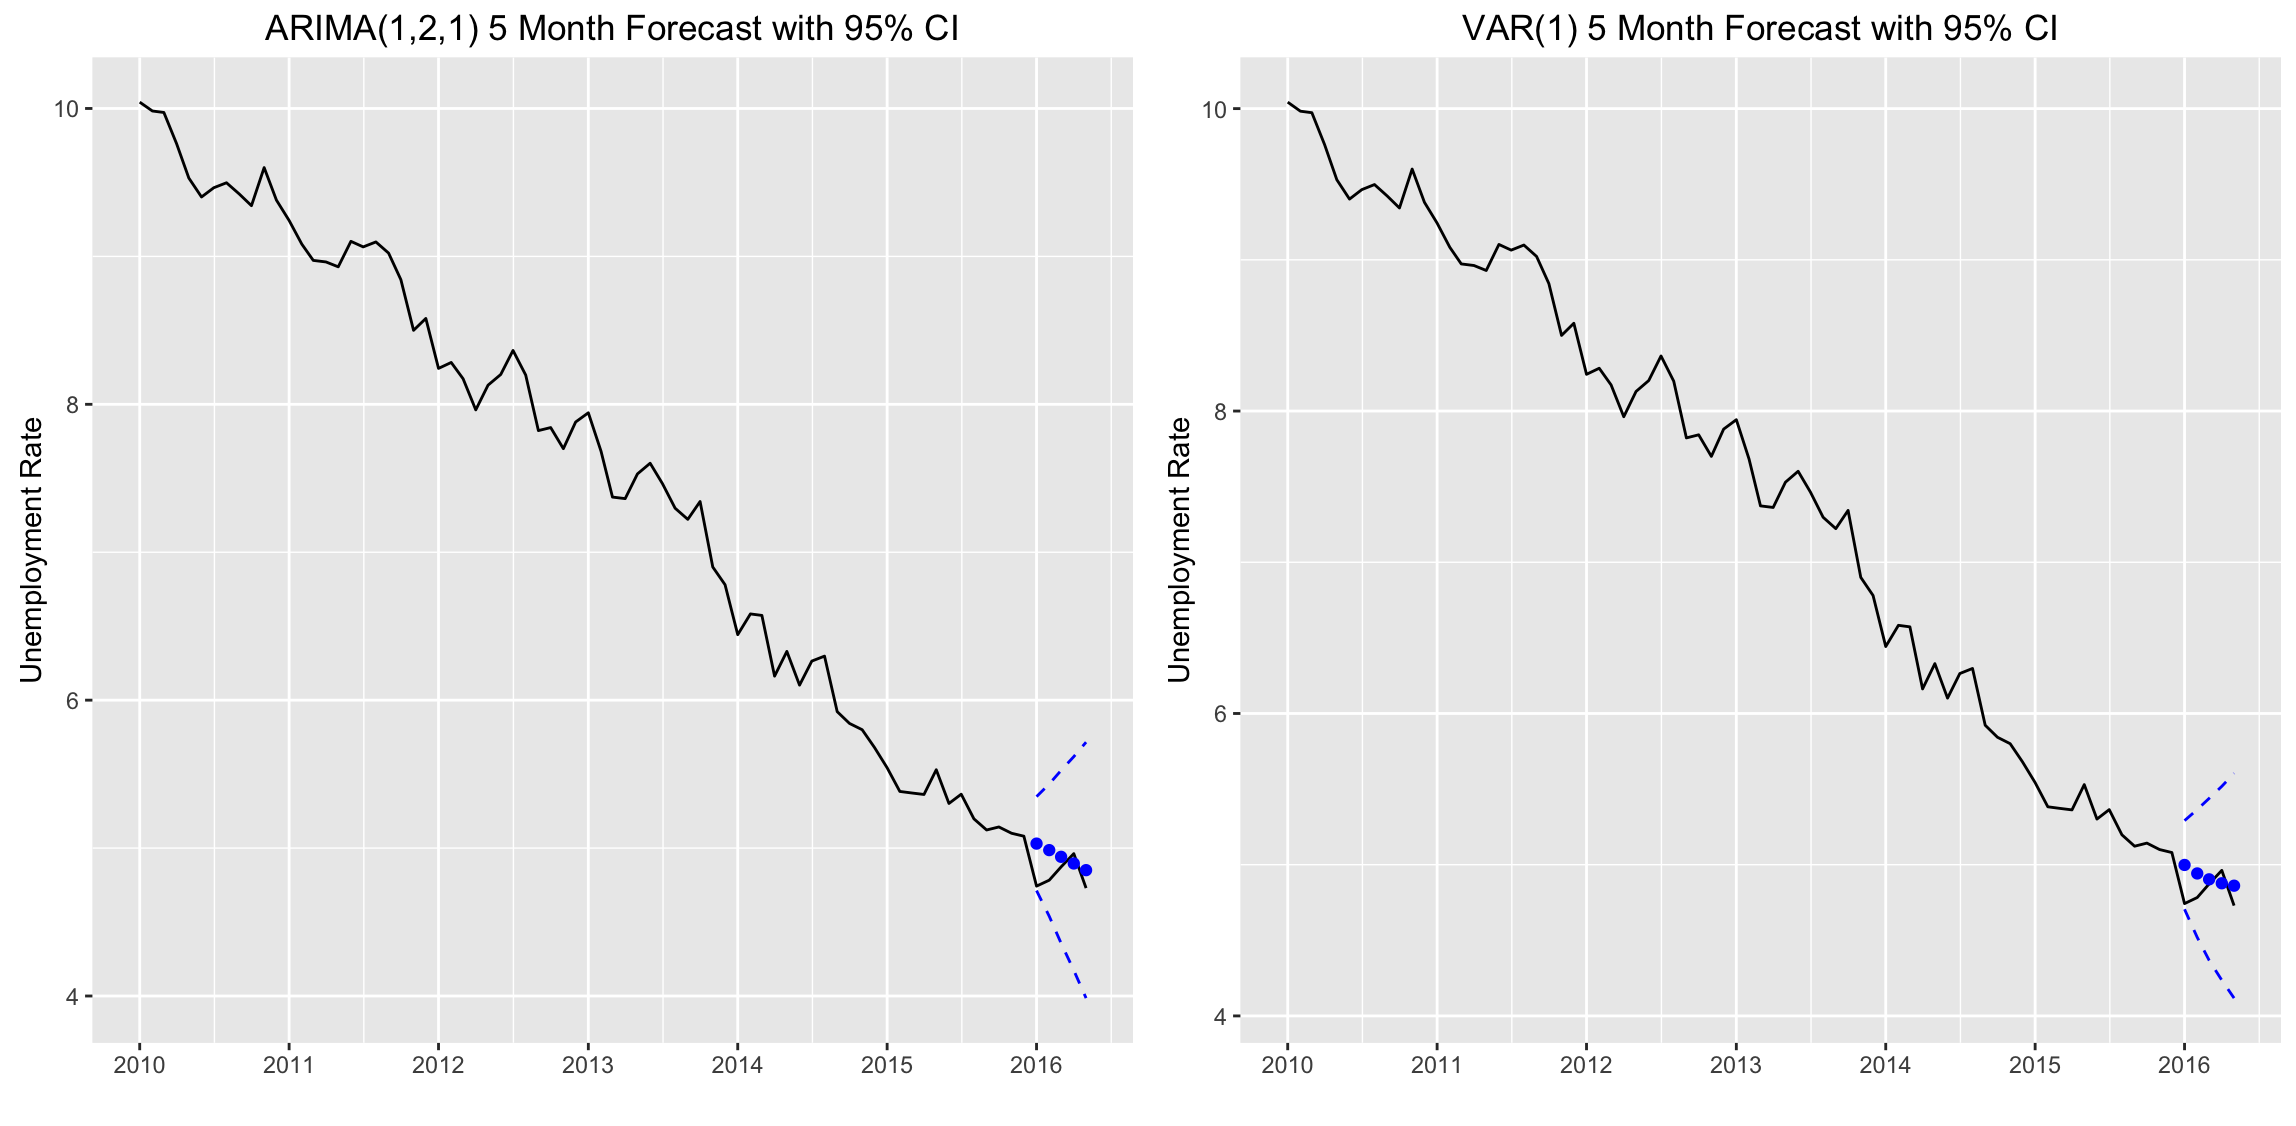
\includegraphics[width=\linewidth]{images/forcasts}
     	\label{fig:forcasts}
      \end{figure}
      
       \begin{figure}[H]
    	\centering
     	\caption{3 year forcasts}
     	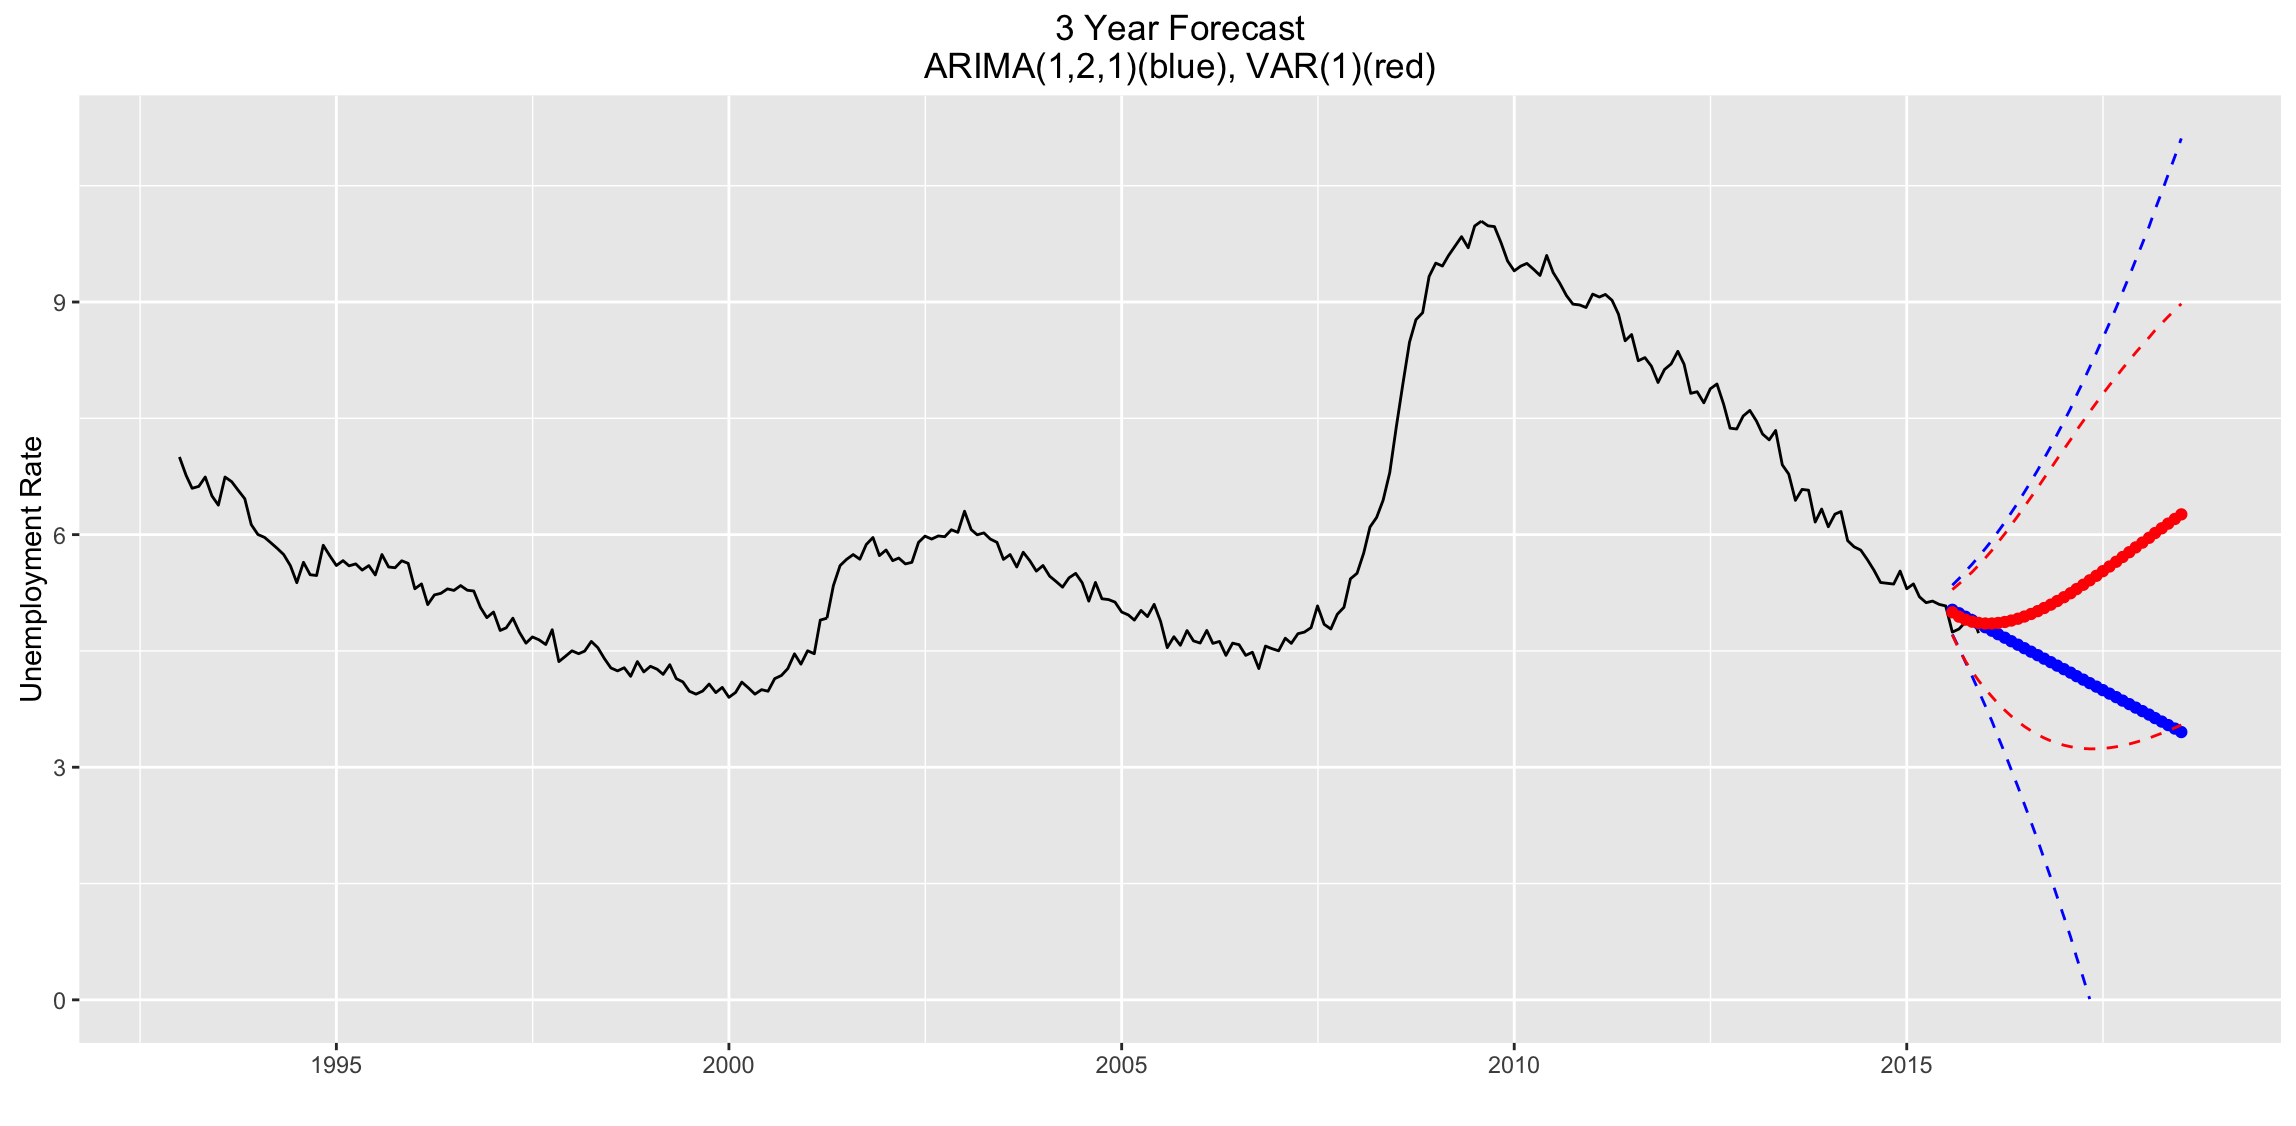
\includegraphics[width=\linewidth]{images/forcast3}
     	\label{fig:forcasts2}
      \end{figure}

\section{Discussion and Implications}

\blindtext % Dummy text

%----------------------------------------------------------------------------------------
%	REFERENCE LIST
%----------------------------------------------------------------------------------------

\begin{flushleft}
\bibliography{main} % refers to our bibliography
\end{flushleft}

\appendix
\section*{Appendix A: Sarima output} \label{App:AppendixA}

       \begin{figure}[H]
    	\centering
     	\caption{Model 1}
     	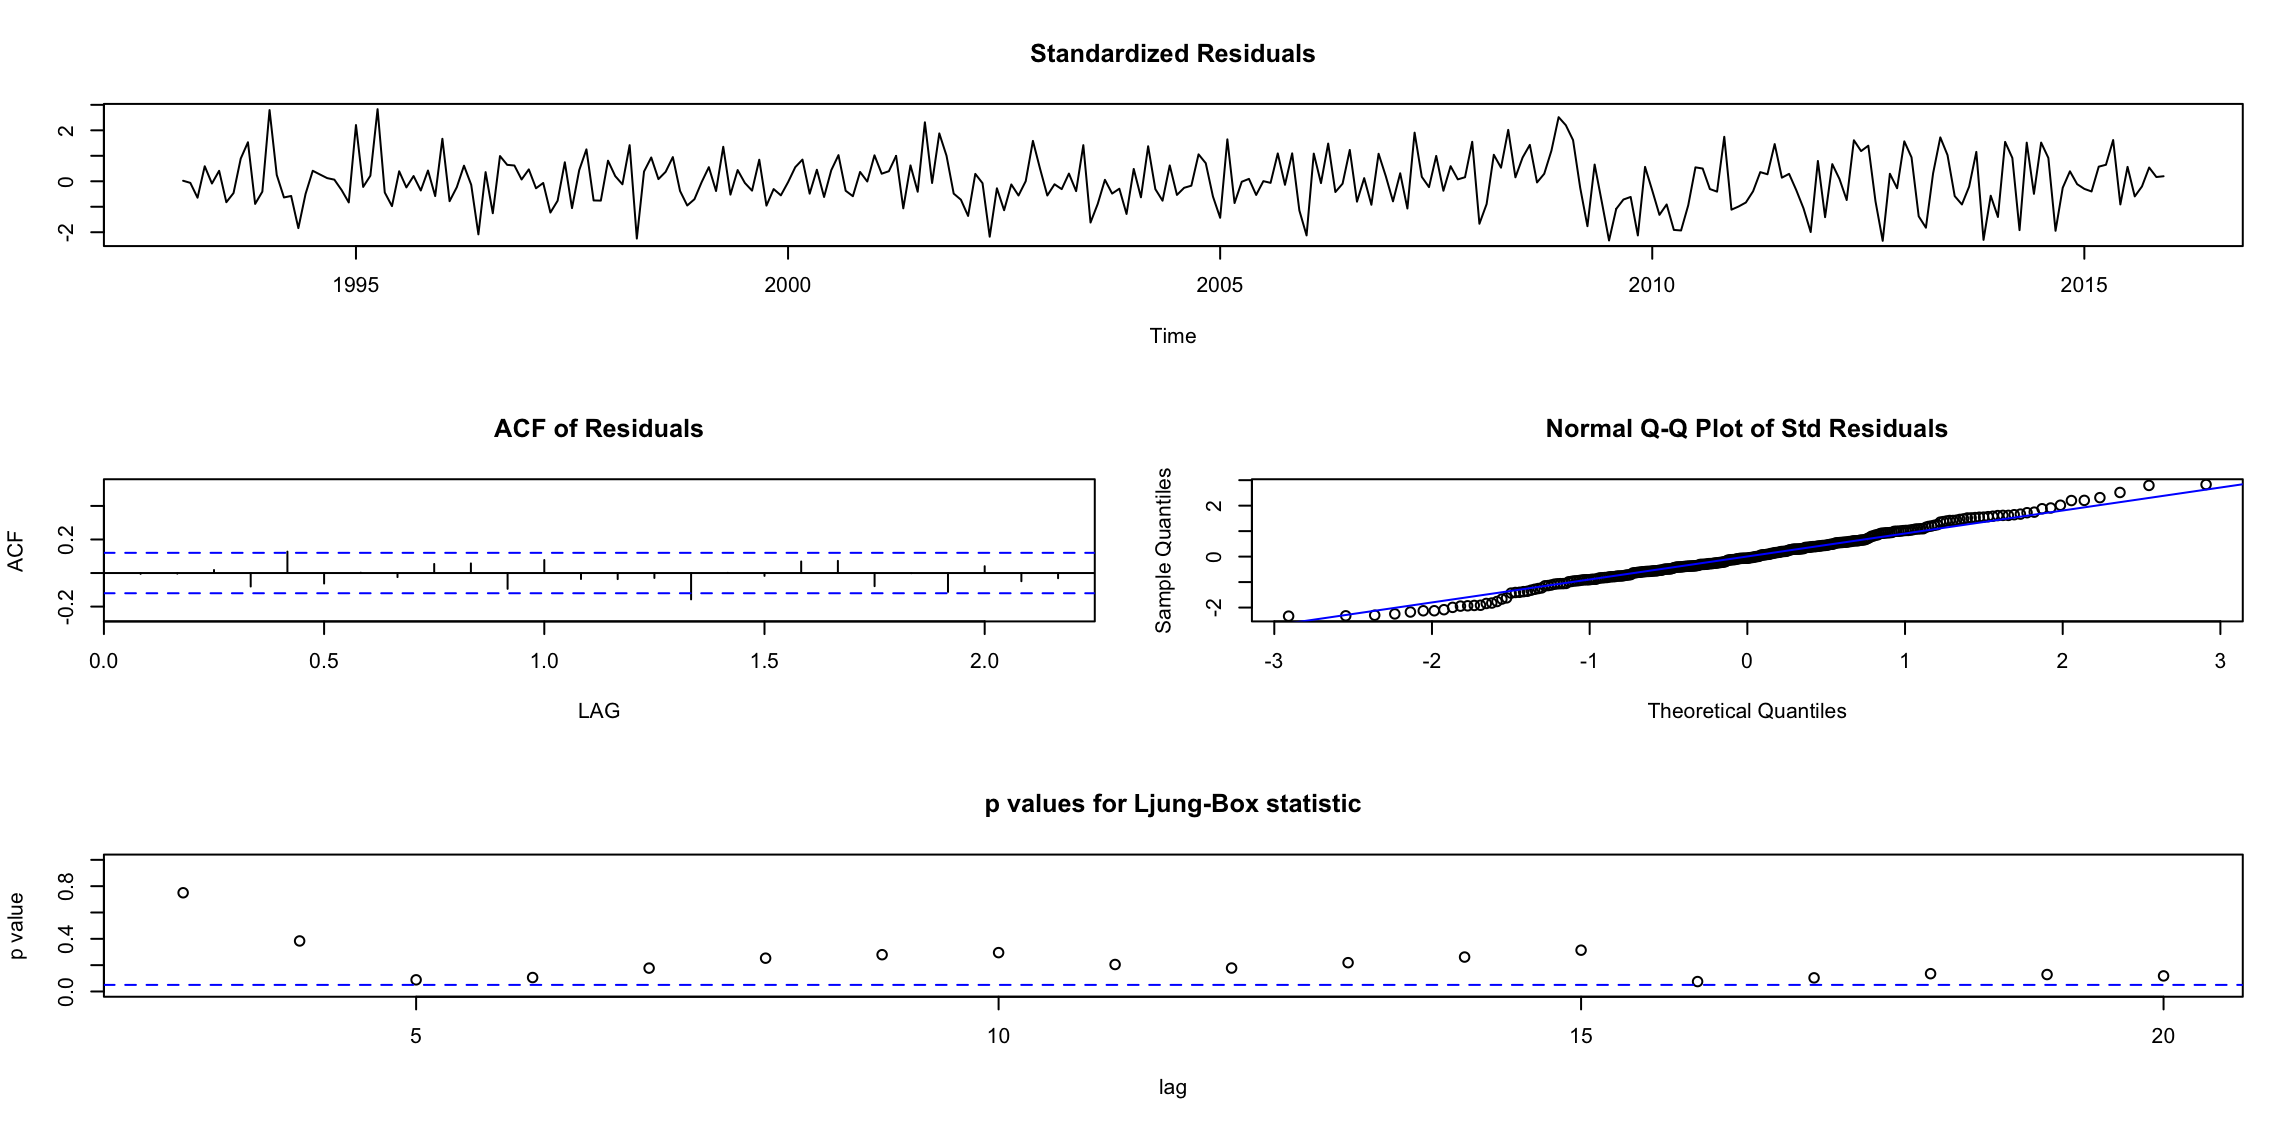
\includegraphics[width=\linewidth]{images/sarima1}
     	\label{fig:sarima1}
     	     	\caption{Model 2}
     	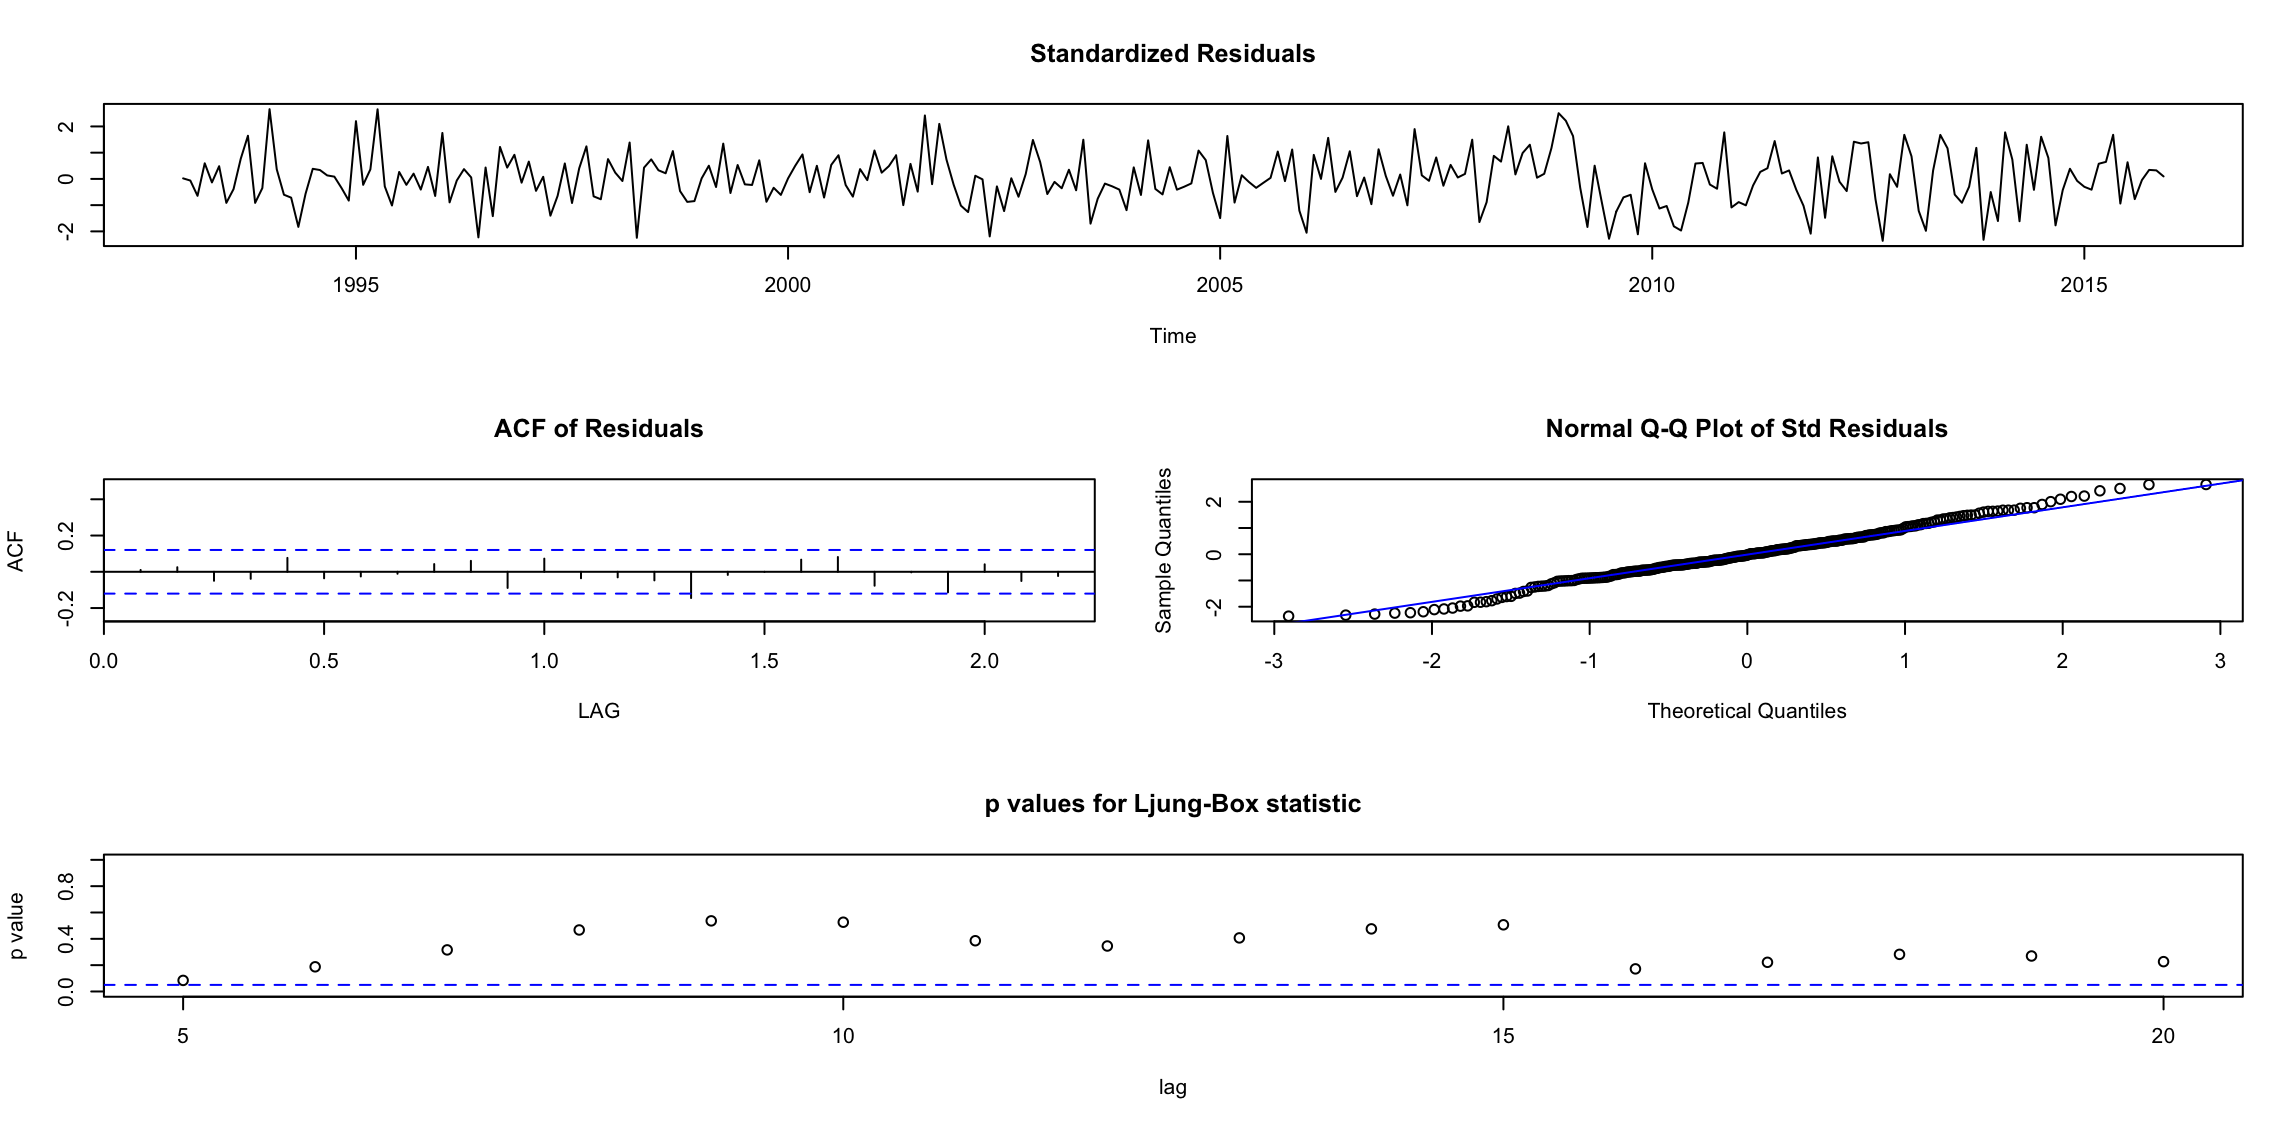
\includegraphics[width=\linewidth]{images/sarima2}
     	\label{fig:sarima2}
     	    	\caption{Model 3}
     	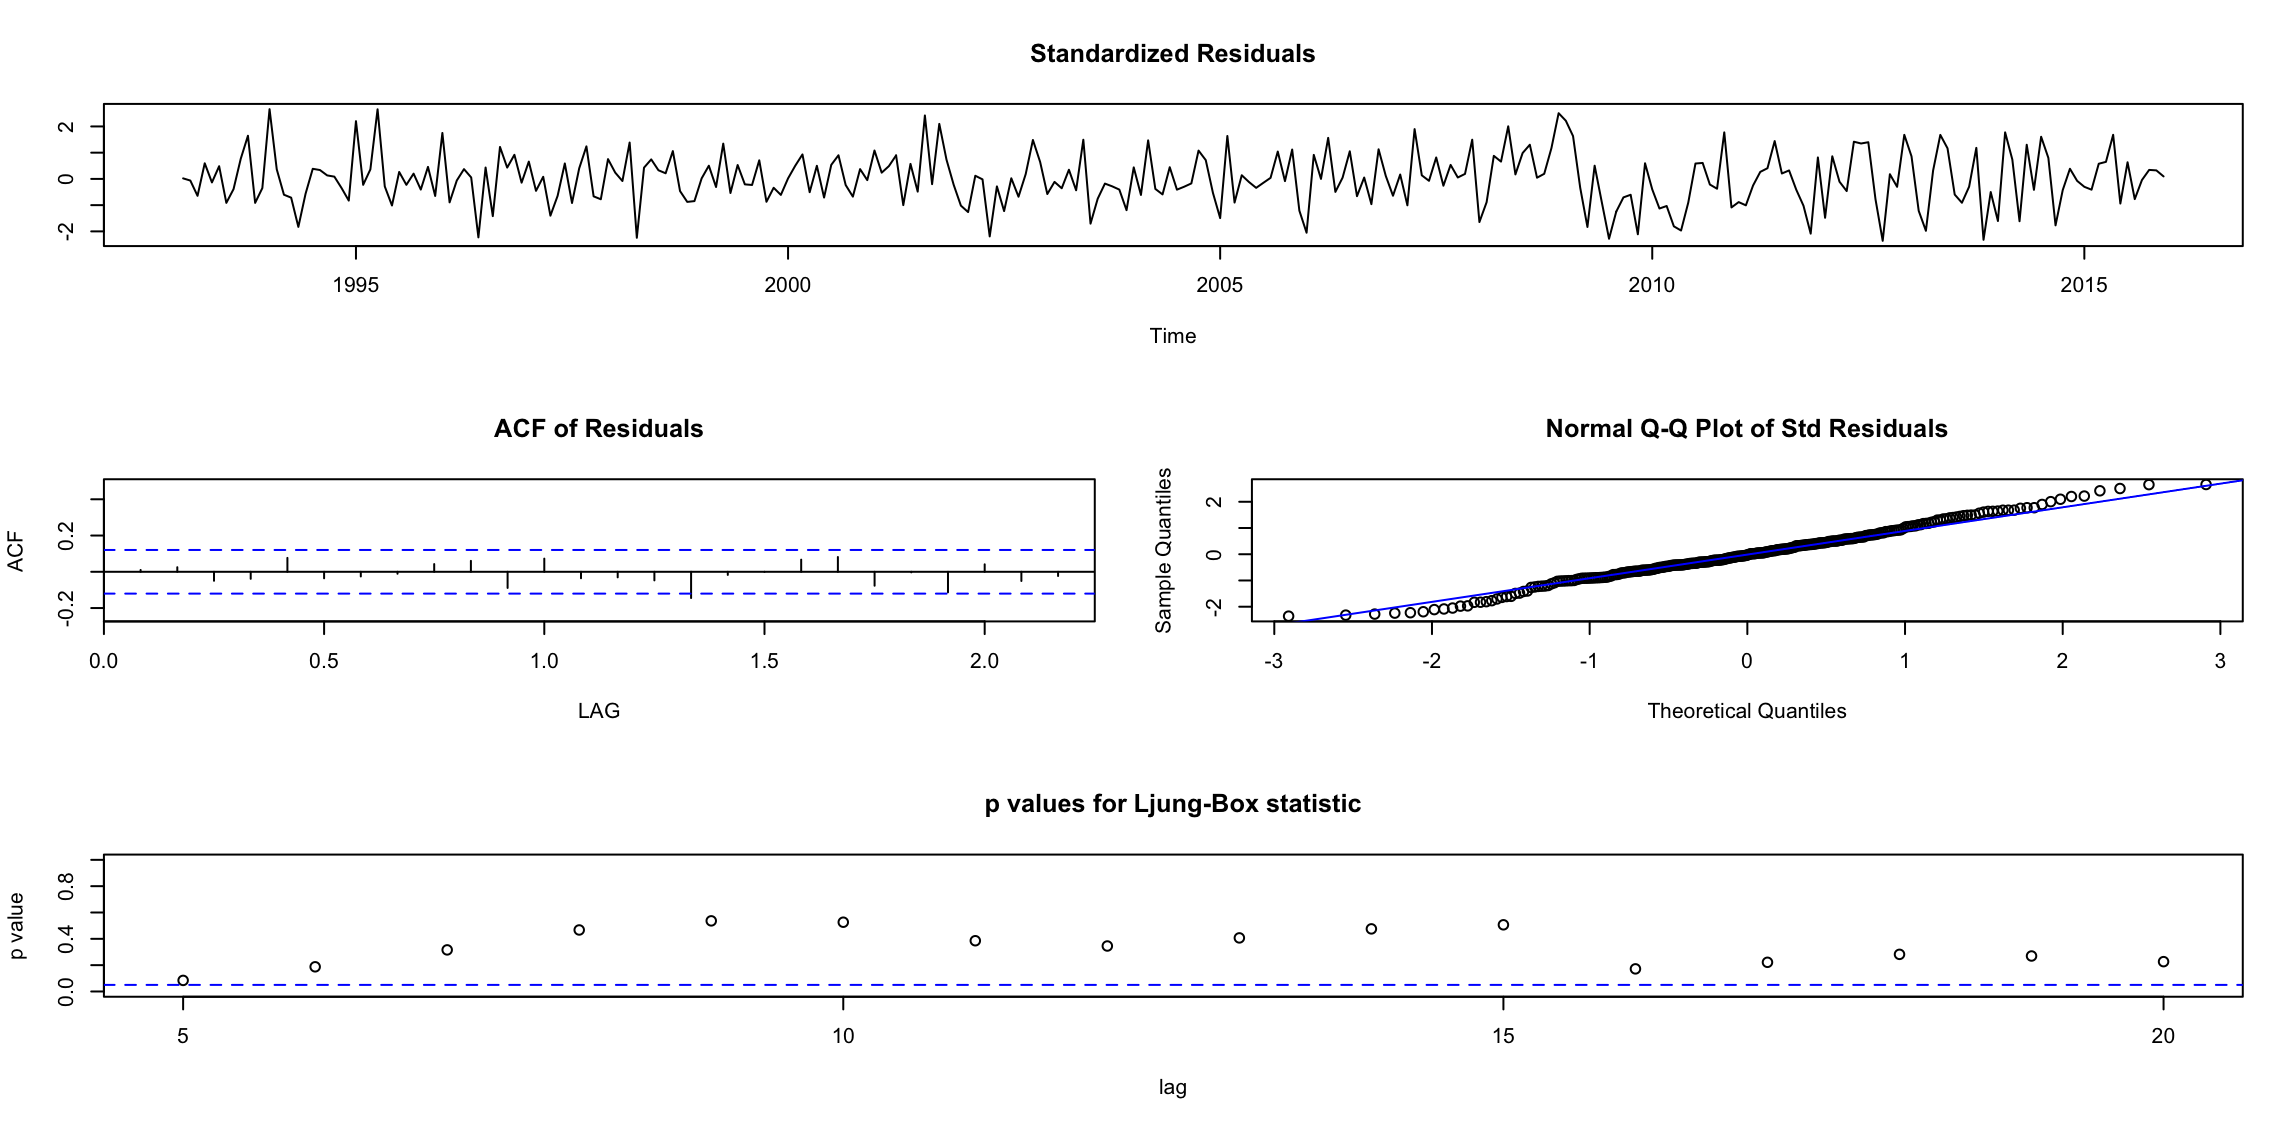
\includegraphics[width=\linewidth]{images/sarima3}
     	\label{fig:sarima3}
      \end{figure}
      
      
      
         \begin{figure}[H]
    	\centering
     	\caption{Model 4}
     	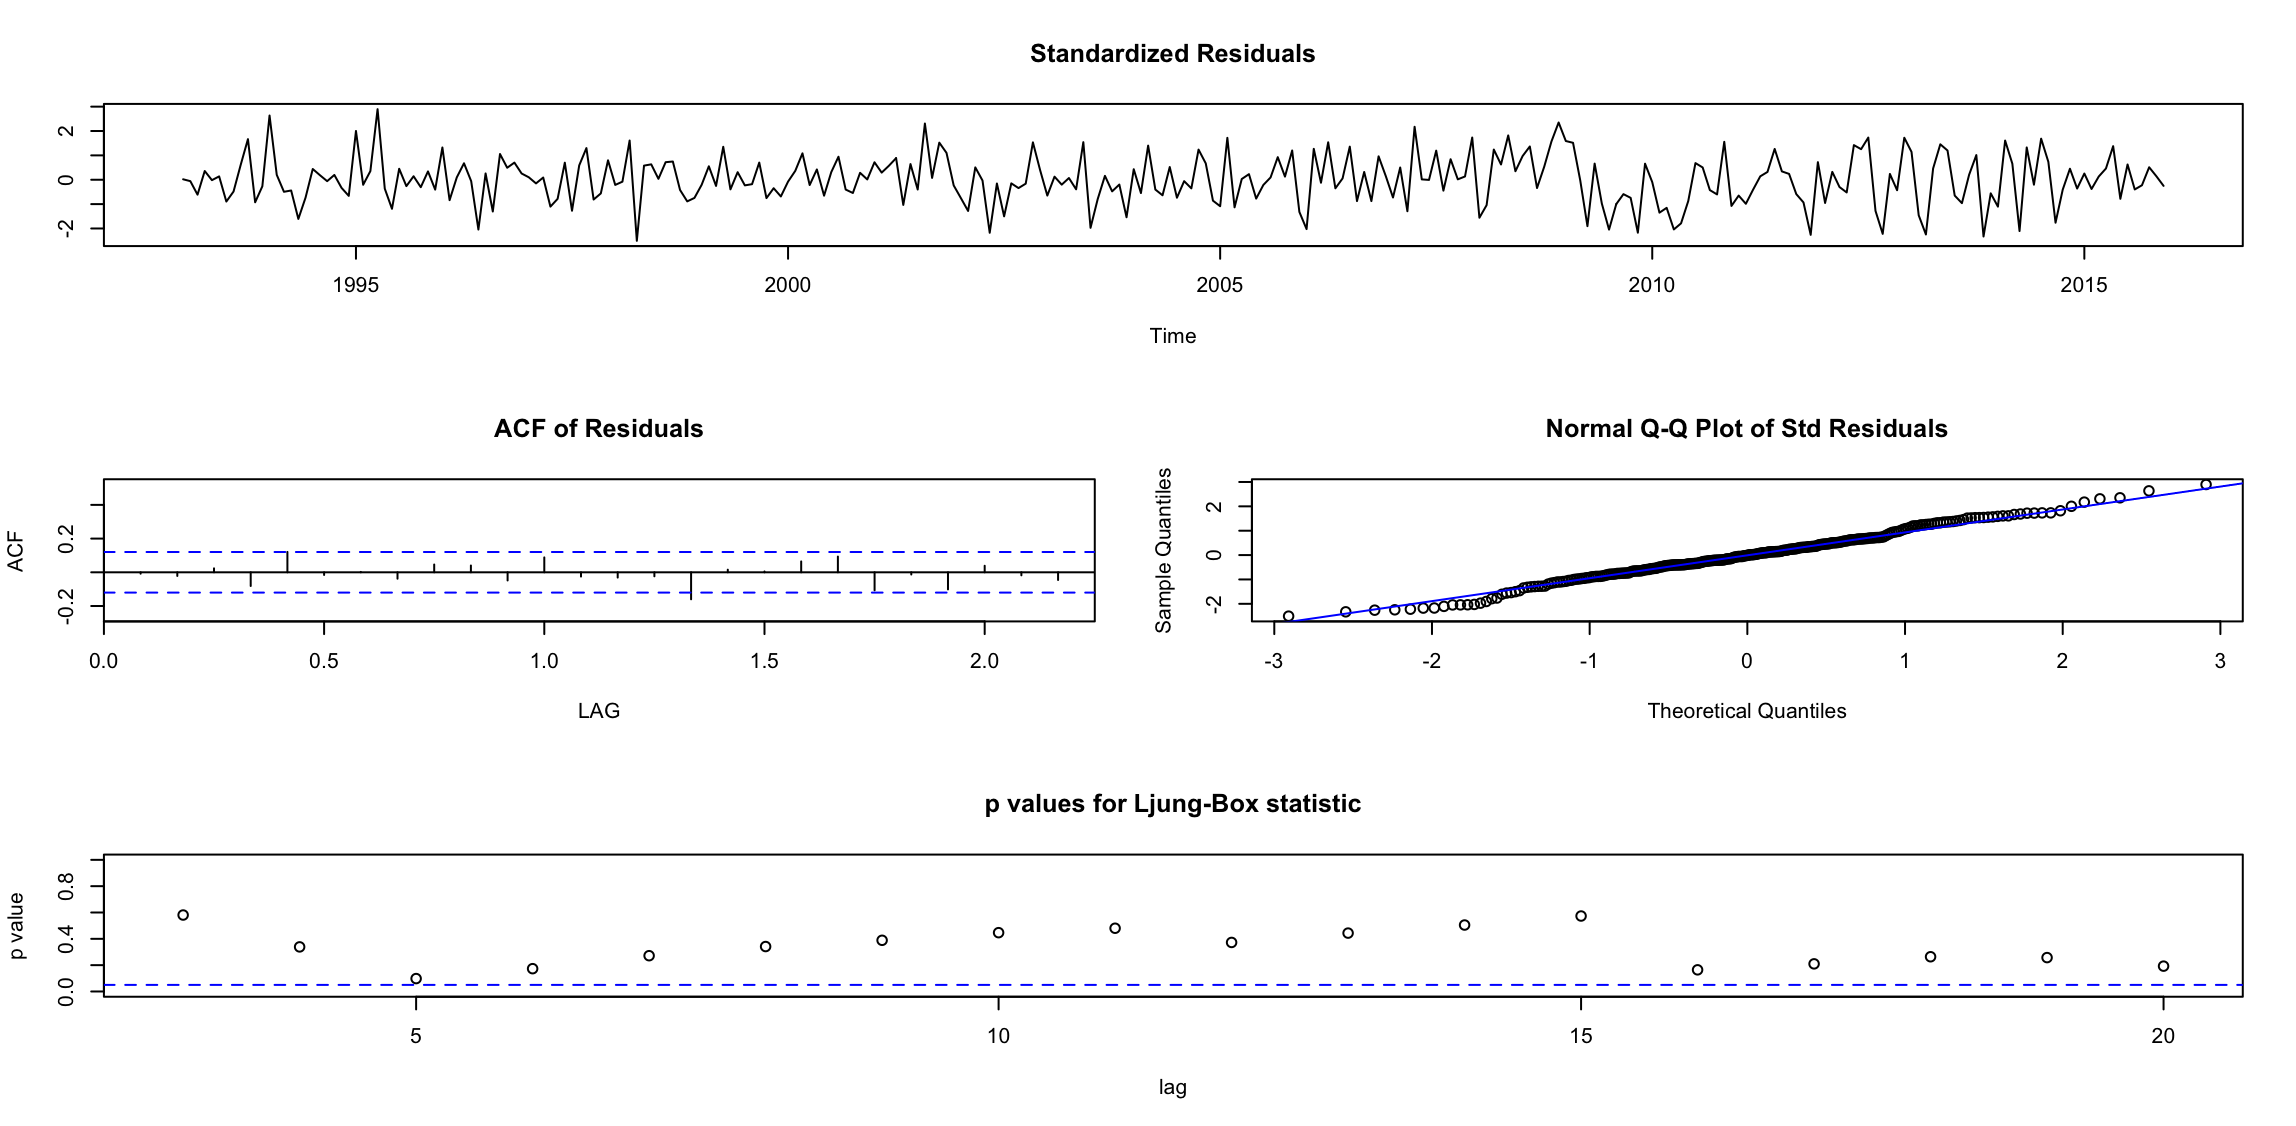
\includegraphics[width=\linewidth]{images/sarima4}
     	\label{fig:sarima4}
     	\caption{Model 5}
     	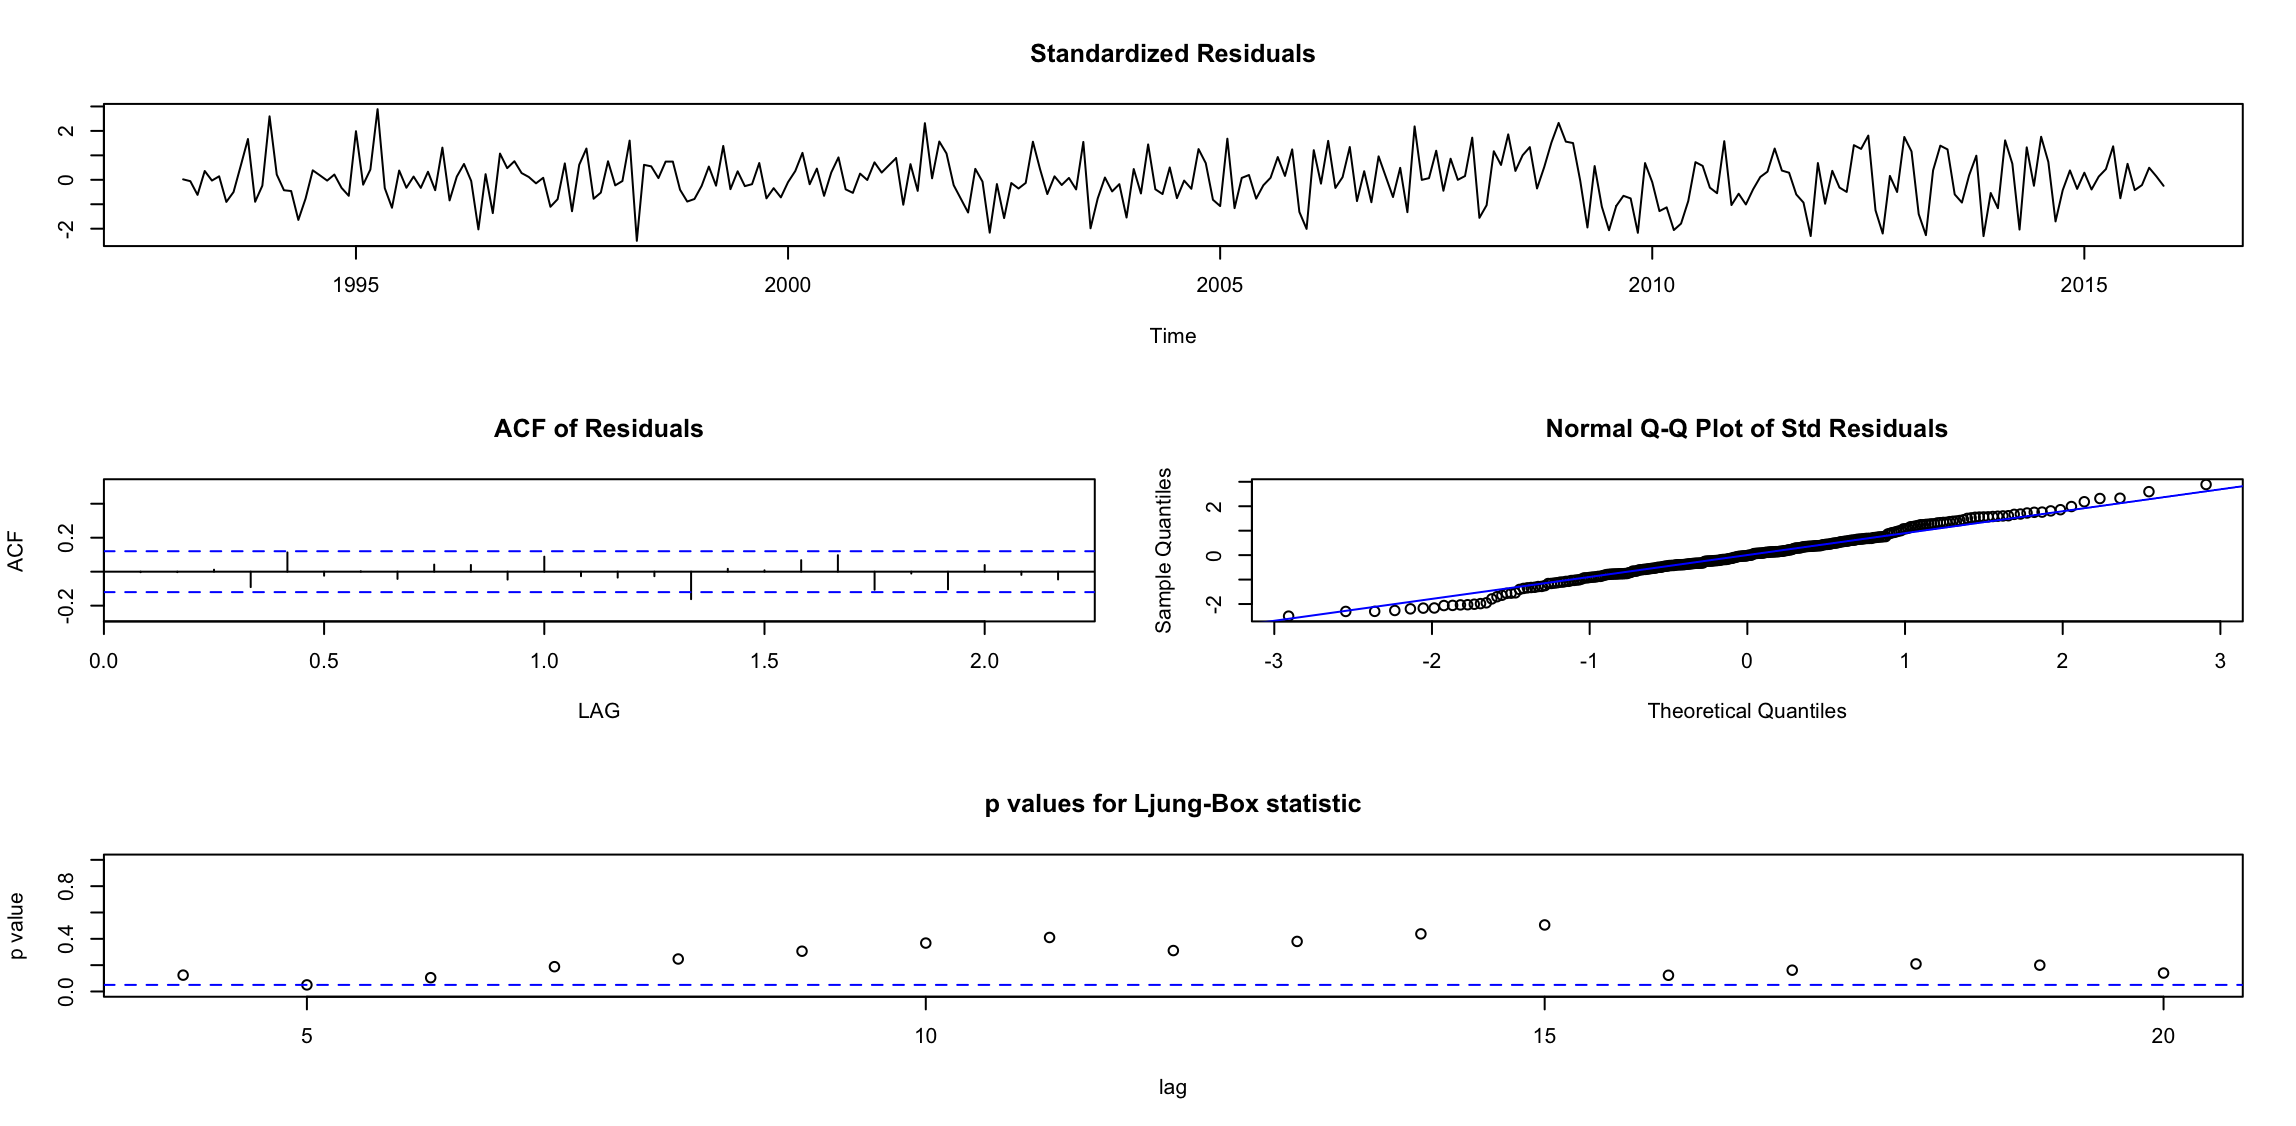
\includegraphics[width=\linewidth]{images/sarima5}
     	\label{fig:sarima5}
     	\caption{Model 6}
     	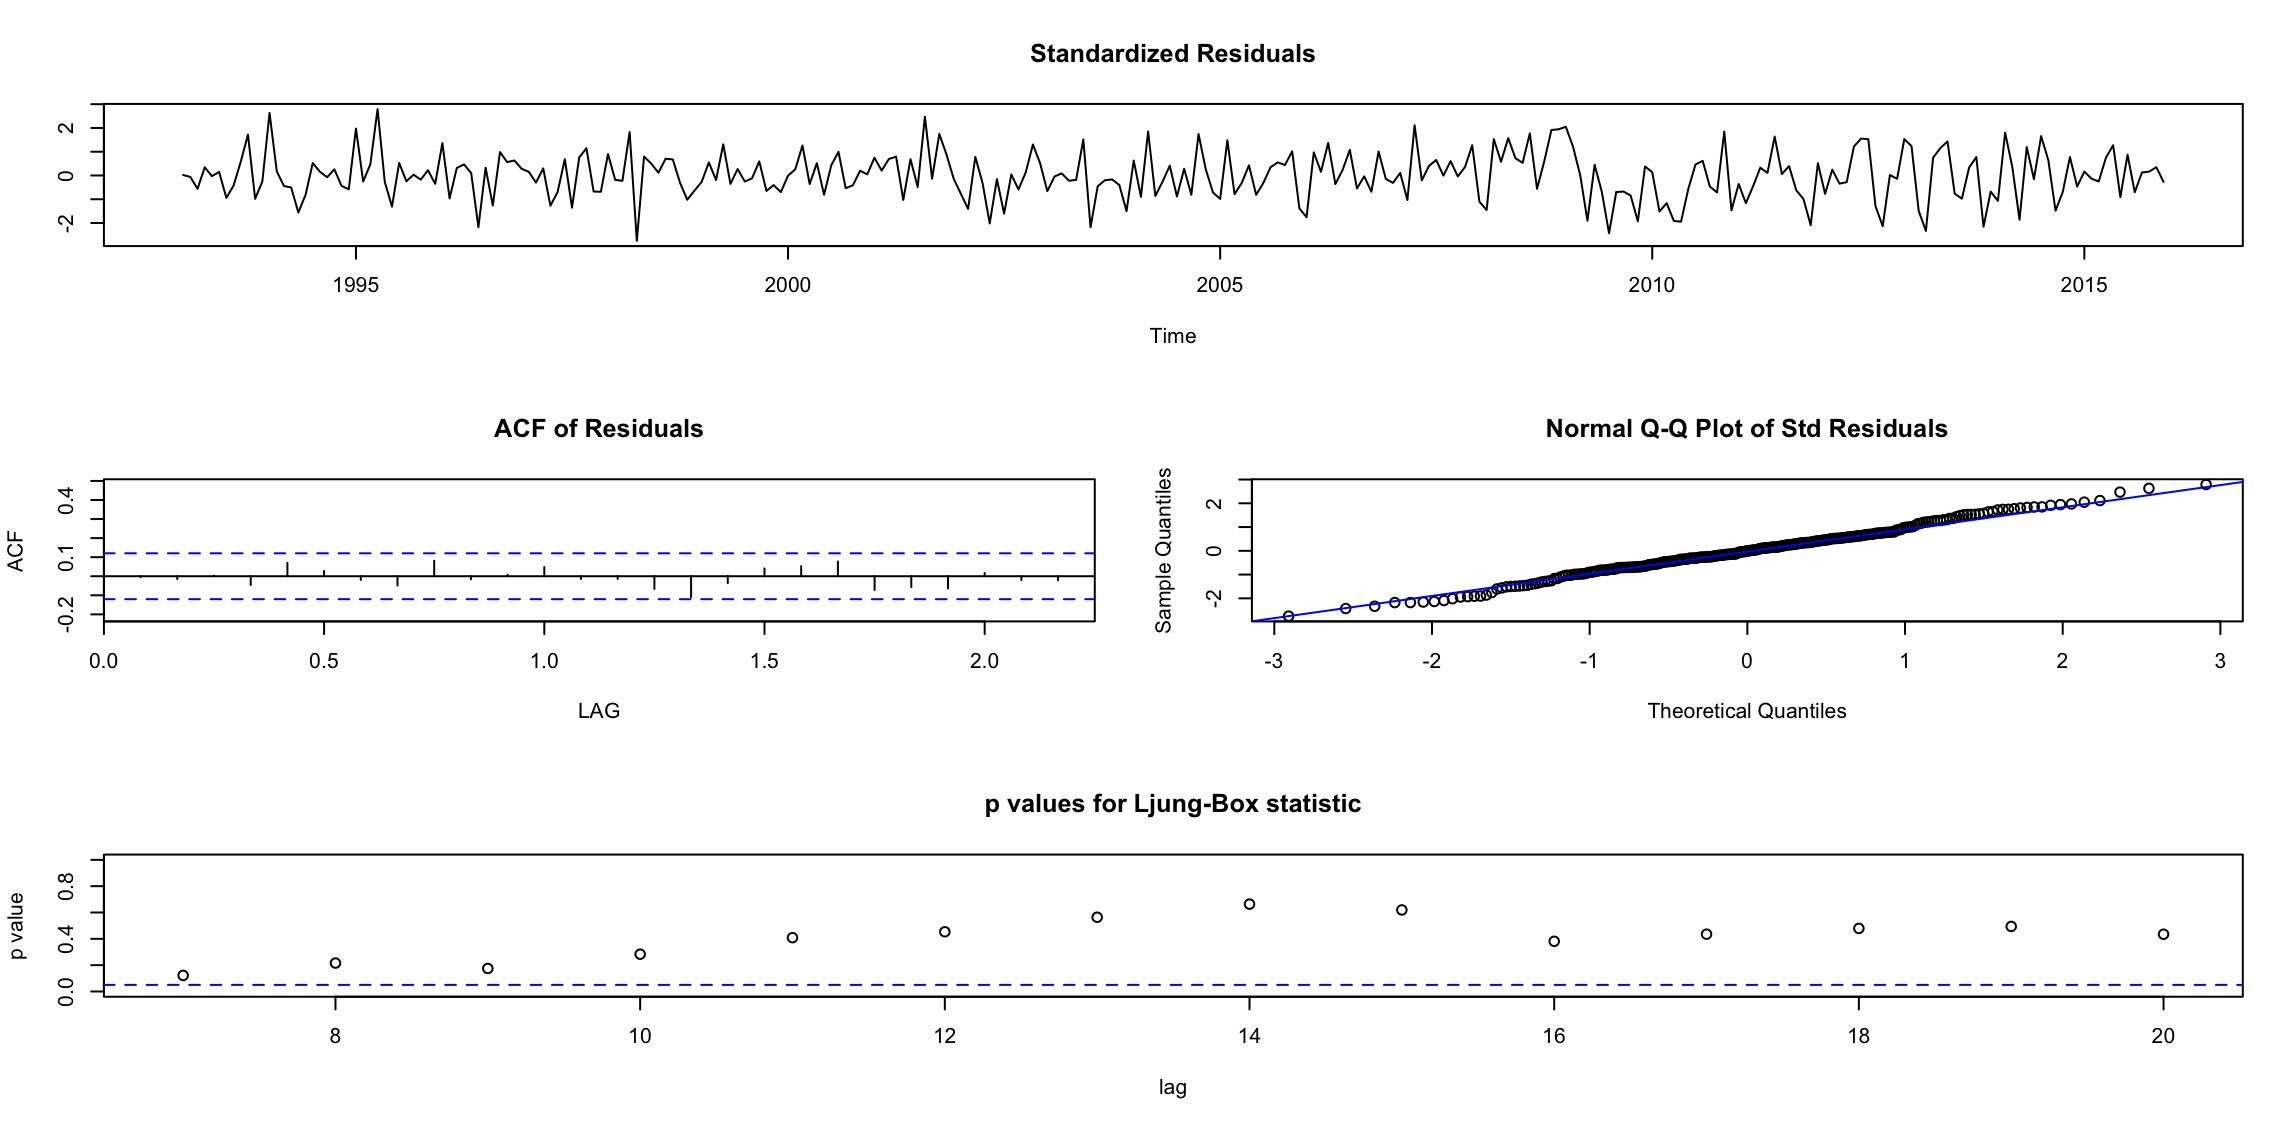
\includegraphics[width=\linewidth]{images/sarima6}
     	\label{fig:sarima6}
     	     	\caption{Model 7}
     	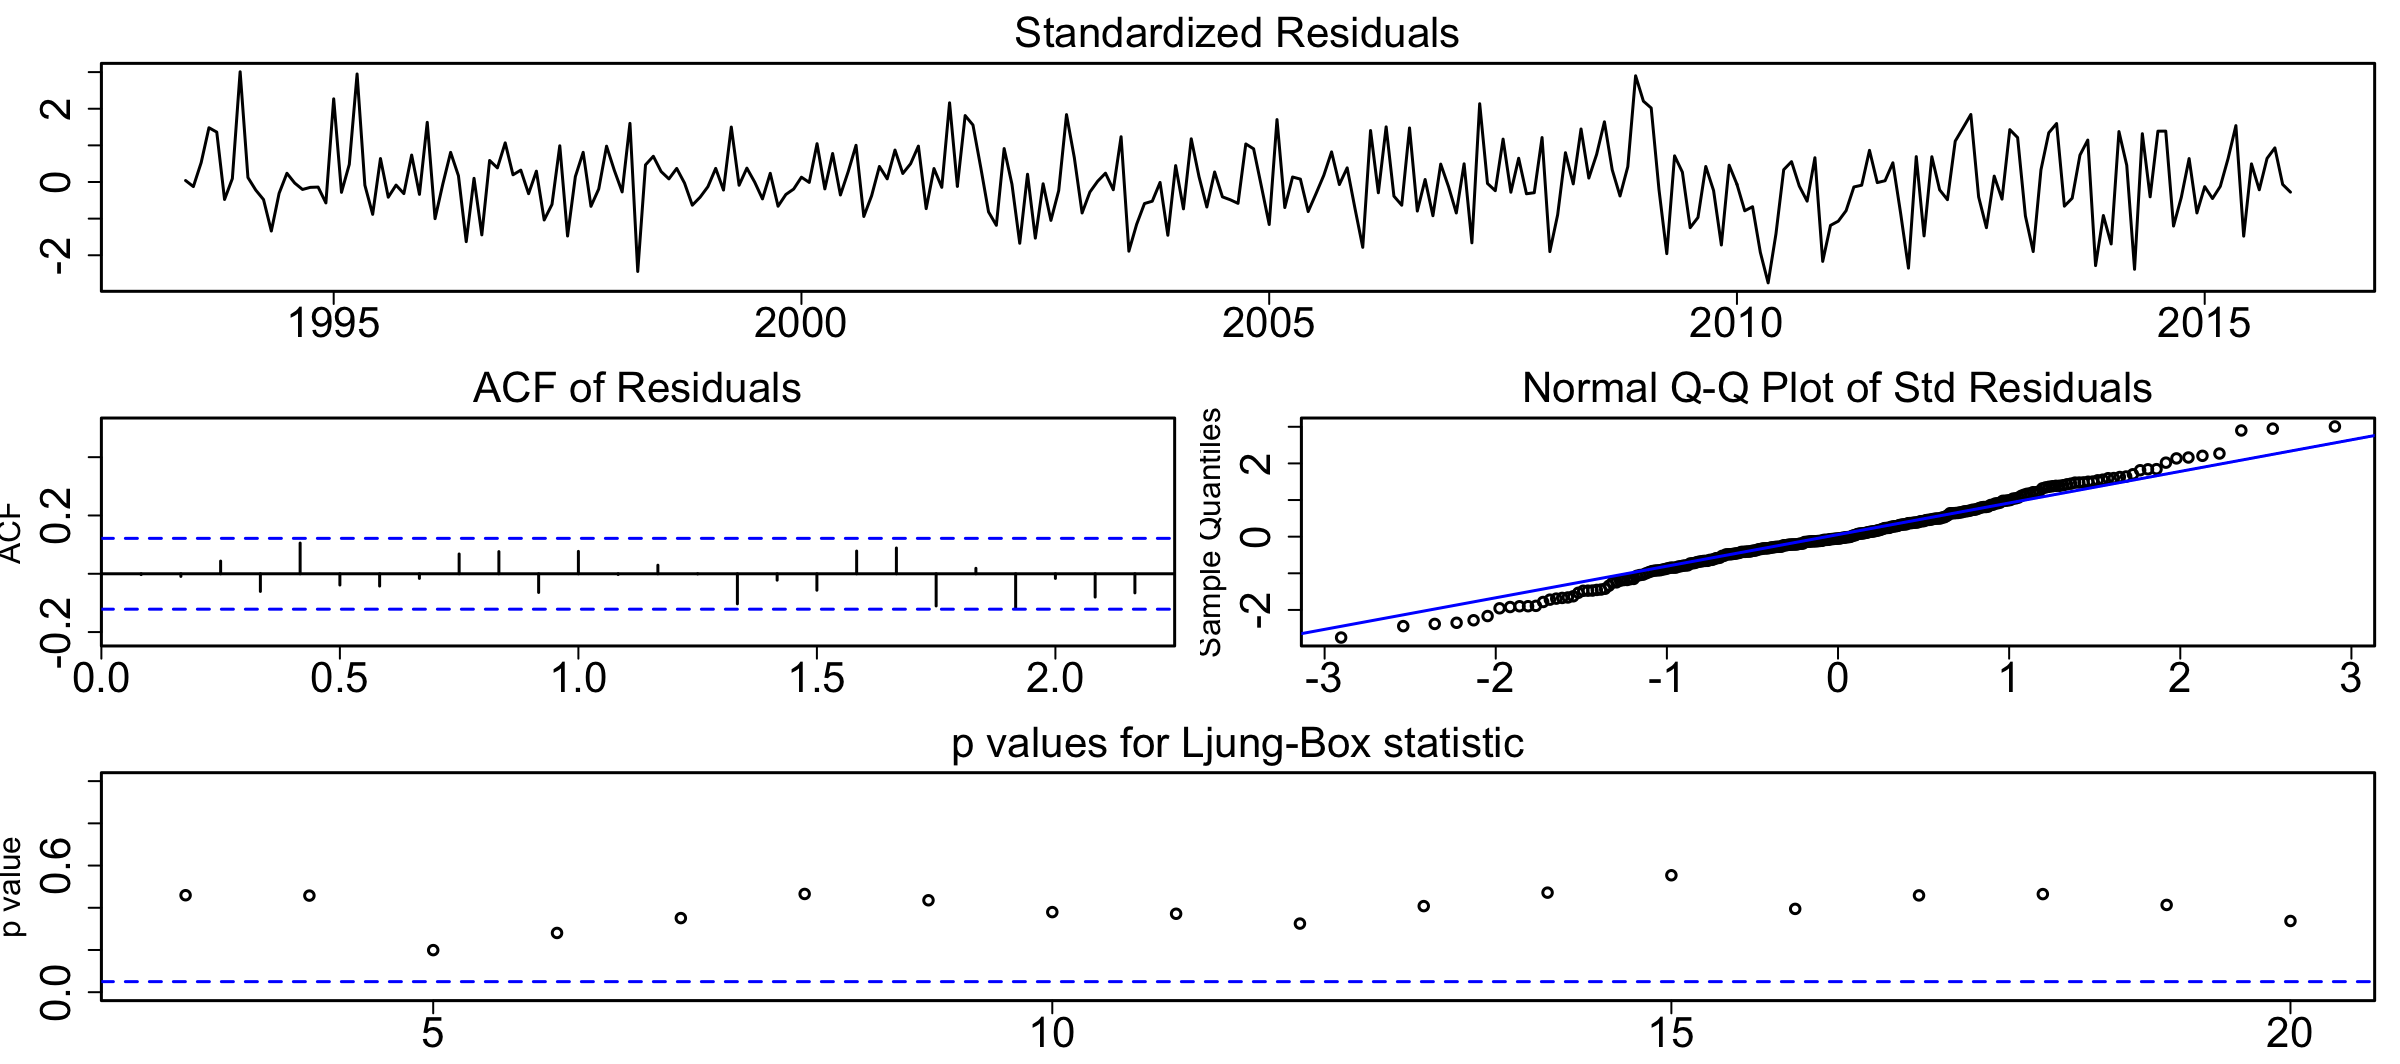
\includegraphics[width=\linewidth]{images/sarima7}
     	\label{fig:sarima7}
      \end{figure}

              \begin{figure}[H]
    	\centering
     	\caption{Model 8}
     	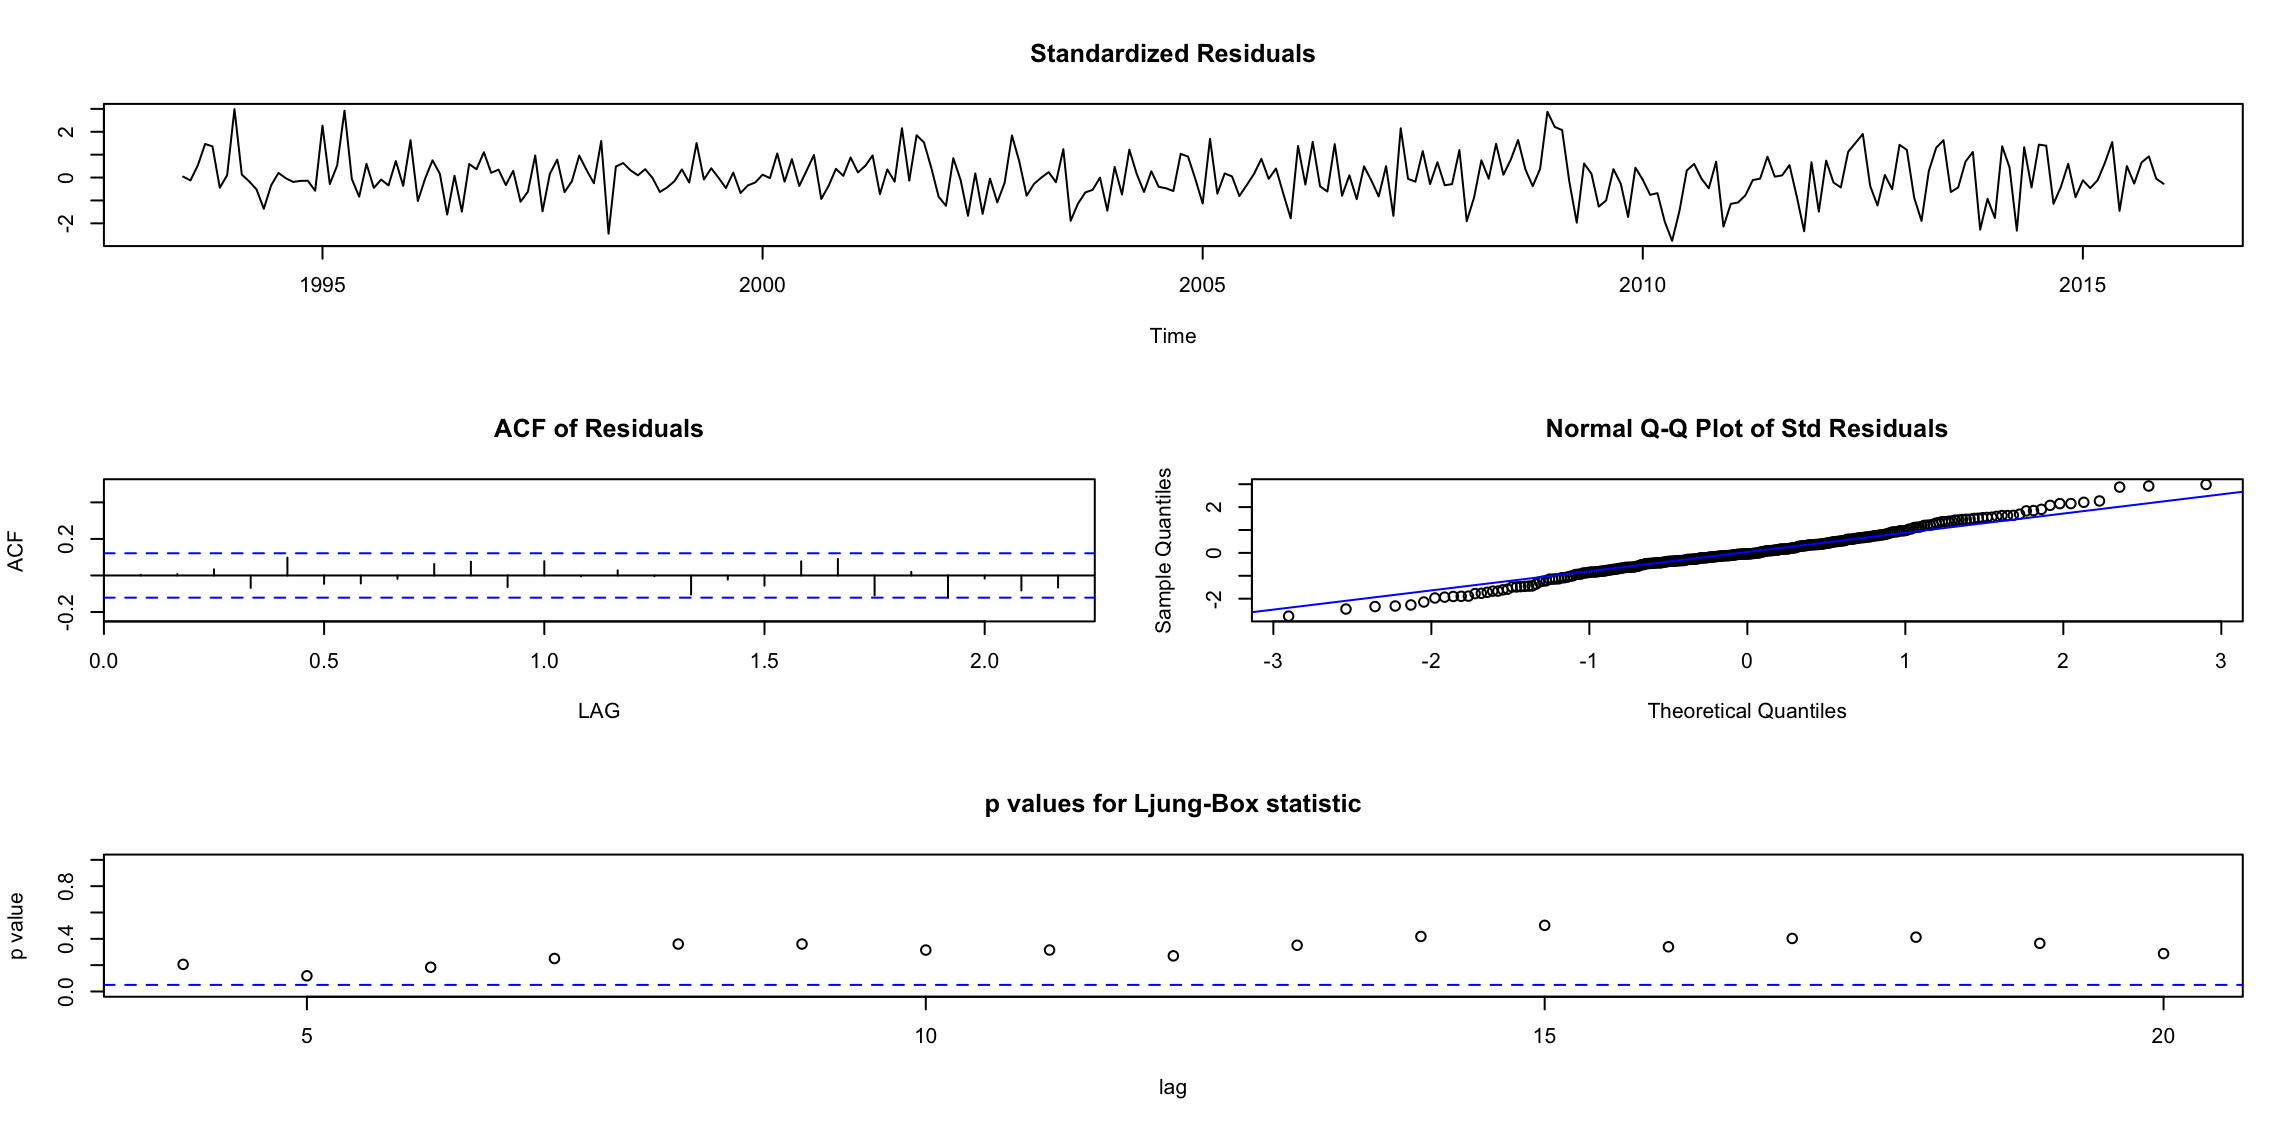
\includegraphics[width=\linewidth]{images/sarima8}
     	\label{fig:sarima8}
     	\caption{Model 9}
     	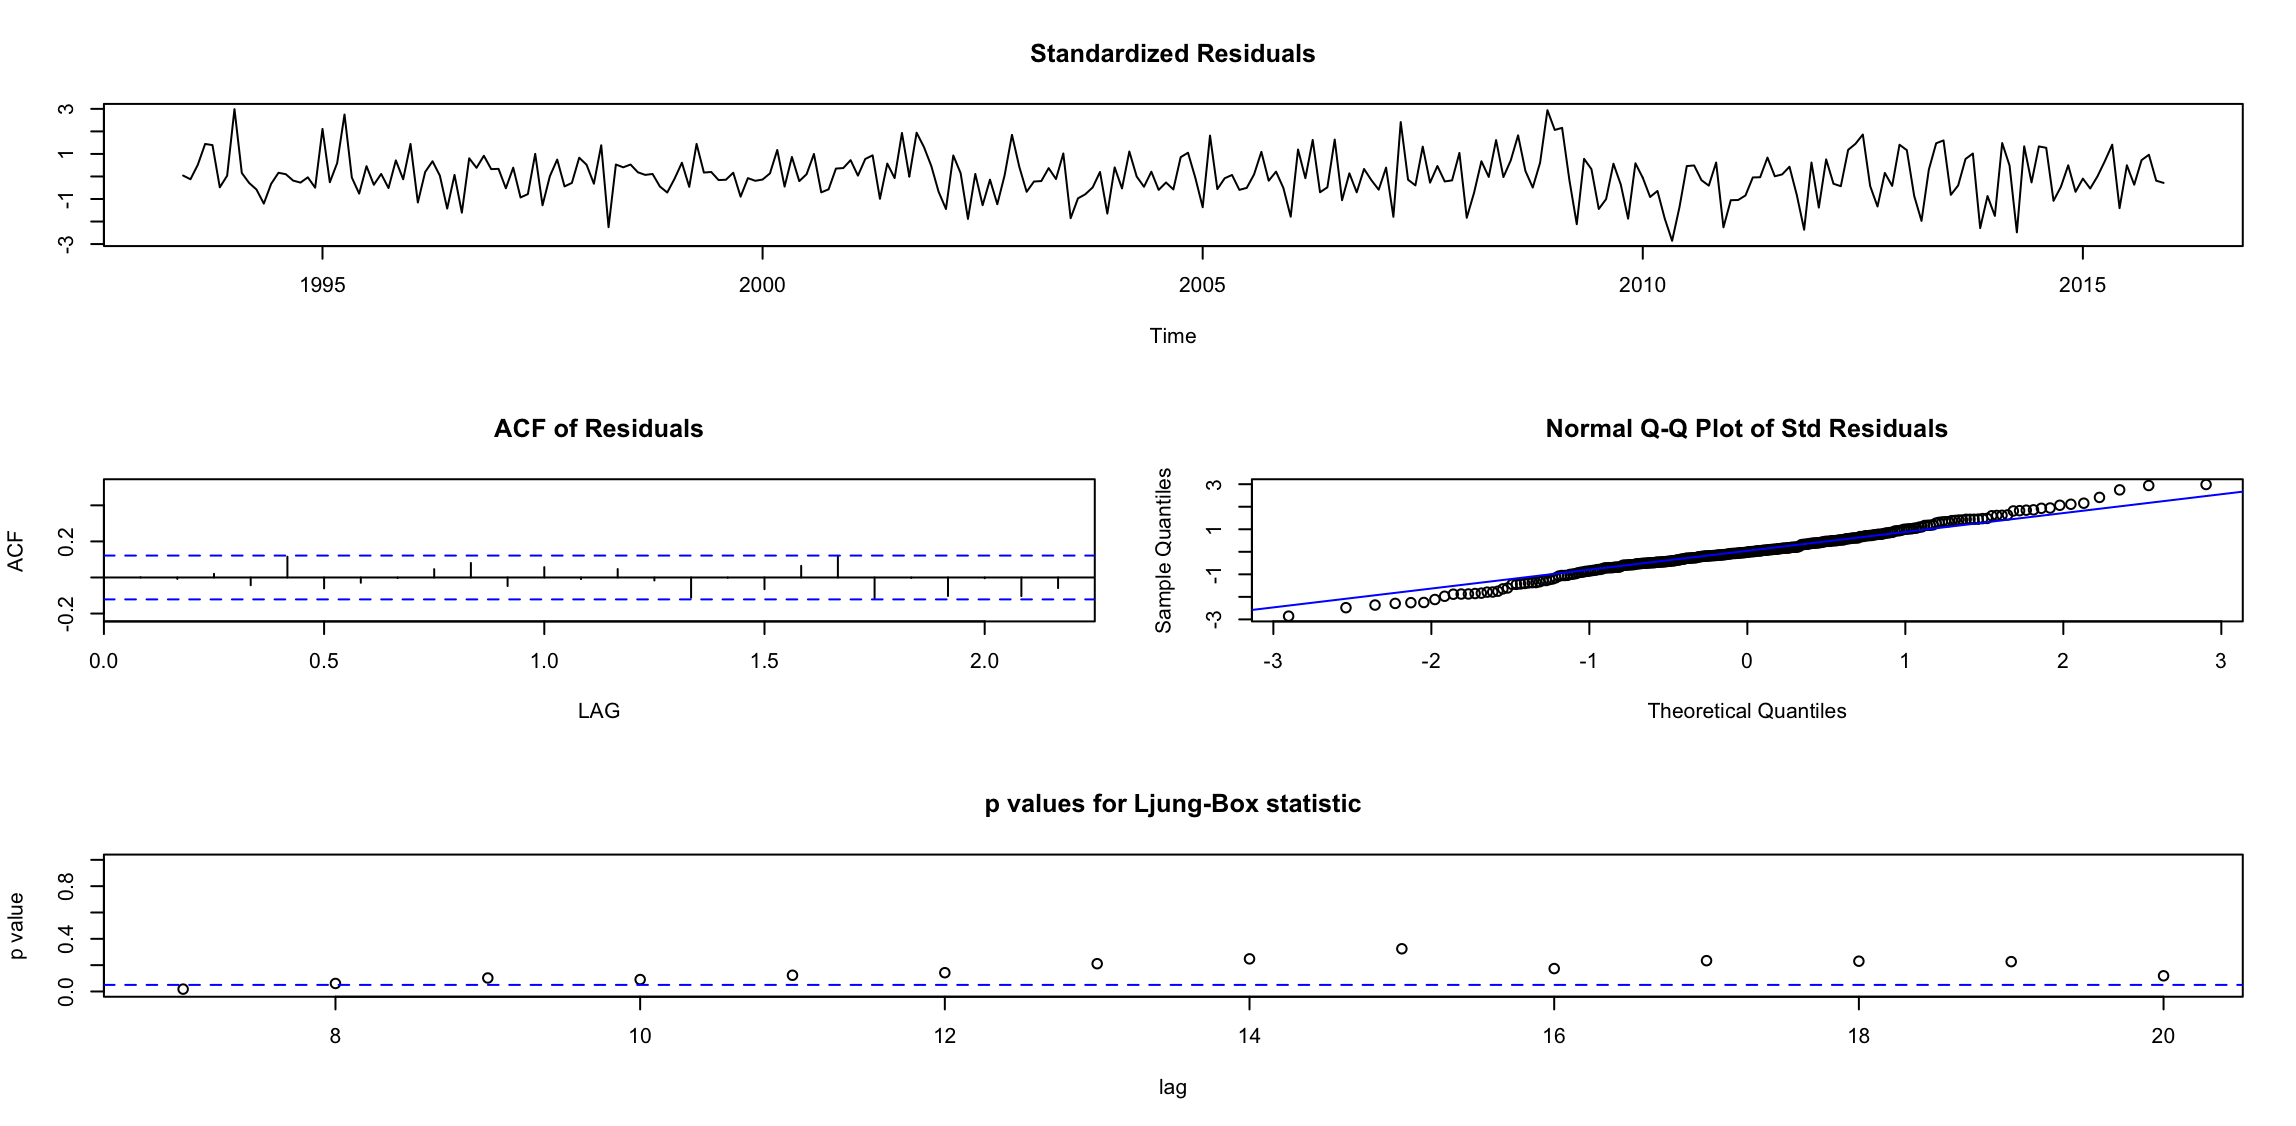
\includegraphics[width=\linewidth]{images/sarima9}
     	\label{fig:sarima9}
      \end{figure}
      
      \section*{Appendix B: Online Discussions}\label{App:AppendixB}
     


Yes, I think we should look at one or two models outside of the current ARIMA set... maybe VAR or Fractional ARIMA. Also @trlilley12 I am unable to run your code without it erroring out so I cannot verify your results.. 



I am glad to start doing some forecasting. I did some with the ARIMA(1, 2, 1) seasonally adjusted, no predictors. It's in the RScript "forecasting."

What other potential models are we considering? My only concern is that if we choose a model with predictors, we will have to forecast those predictors before we forecast the unemployment rate.

In case we go with the ARIMA(1, 2, 1) model for the seasonally adjusted data with no predictors, here are some forecast plots. I uploaded them in the Plots folder, too.

The graphs are for the h = 5, 12, and 24 step ahead forecasts. The first three were generated by sarima( ), and the last three by Arima( ). Personally, I think the last three look better. I think it's good to have a picture of the forecast in the context of all the data. I will play around with sarima( ) to see if I can adjust the default axes to accommodate all past data.


 \begin{figure}[H]
    	\centering
     	\caption{Plots described above}
     	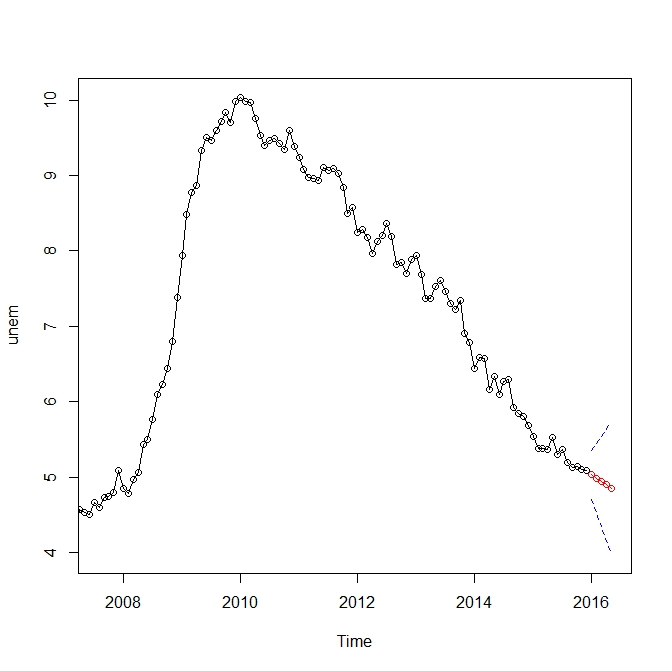
\includegraphics[width=.9\linewidth]{images/fore1}
 \end{figure}
 
  \begin{figure}[H]
    	\centering
     	\caption{Plots described above}
     	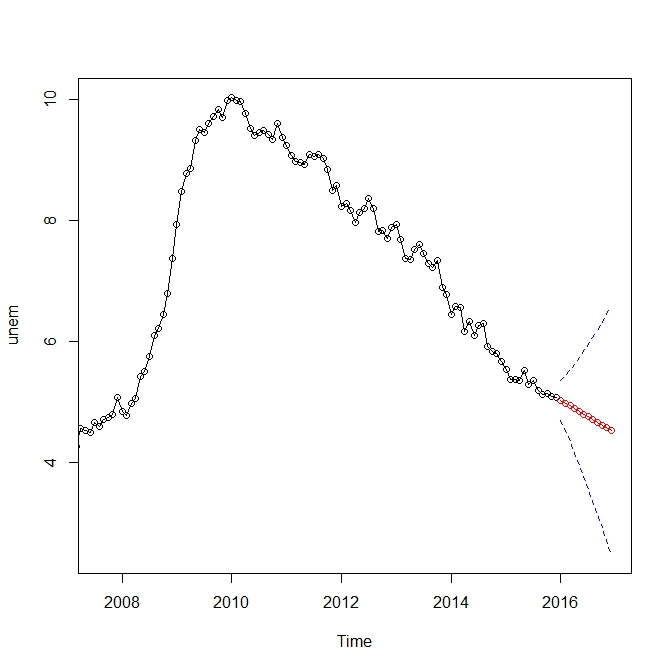
\includegraphics[width=.9\linewidth]{images/fore2}
     	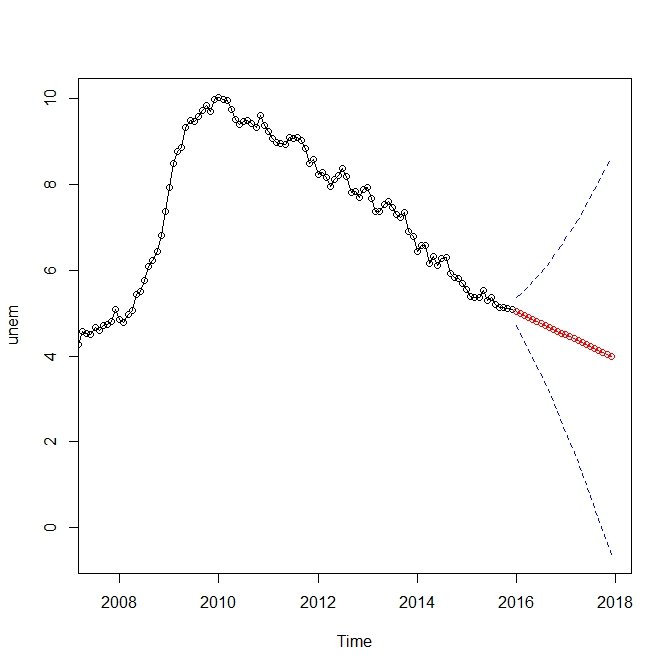
\includegraphics[width=.9\linewidth]{images/fore3}
     	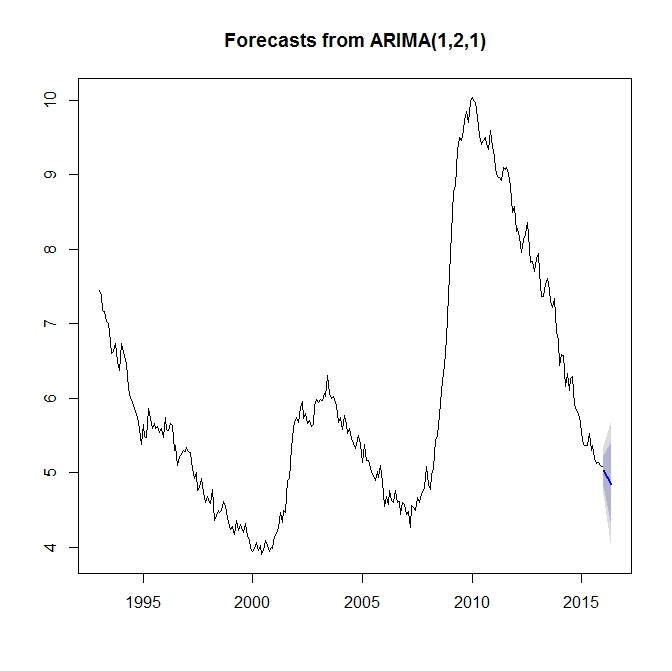
\includegraphics[width=.9\linewidth]{images/fore4}
 \end{figure}

  \begin{figure}[H]
    	\centering
     	\caption{Plots described above}
     	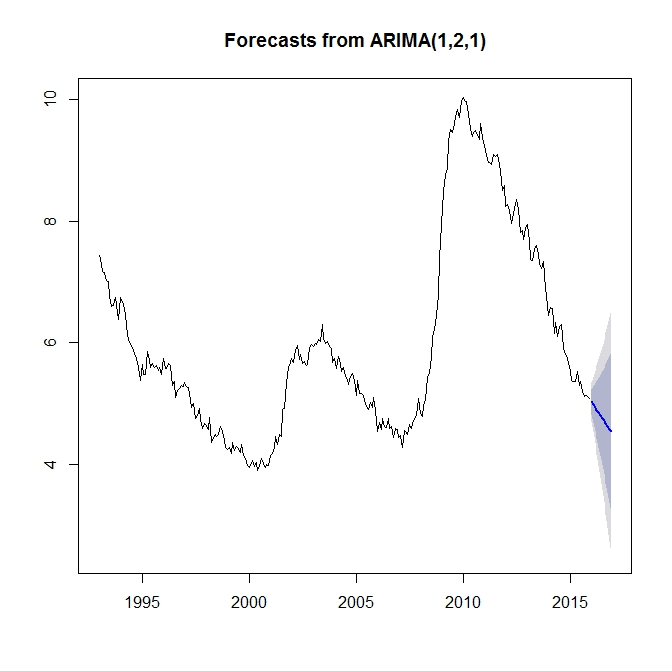
\includegraphics[width=.8\linewidth]{images/fore5}
     	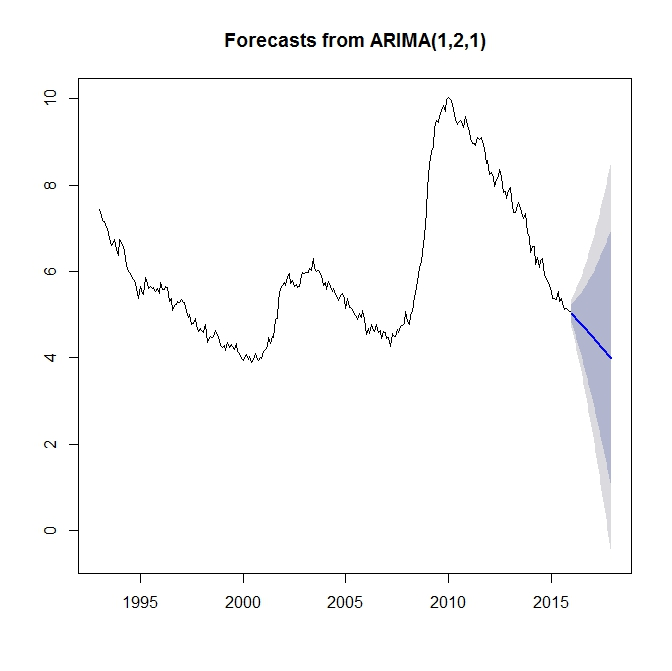
\includegraphics[width=.7\linewidth]{images/fore6}
     	\caption{Plot described below}
     	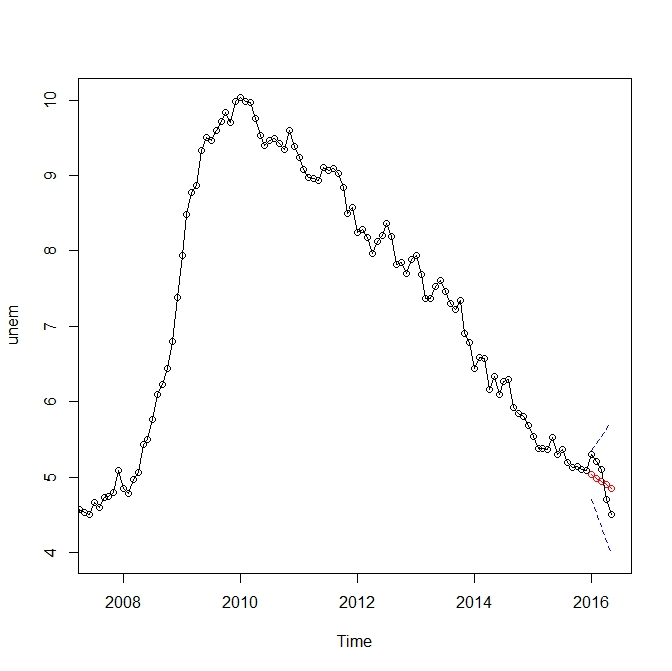
\includegraphics[width=.7\linewidth]{images/fore7}
 \end{figure}
 
 And here is a plot of the first five forecasted values (red) along with the actual observed values (black) from 2016. 
 
 I looked at the FRED website where we got our data, and it looks like the unemployment for June 2016 has been posted at 5.1\%. We could compare that to our predictor for June 2016 as well.

Here is a plot from Arima( ) that shows the predicted values through June 2016 (blue) and the observed values (black).

I put all the code for my plots in the RSCript folder and named it ``forecasting plots.''

  \begin{figure}[H]
    	\centering
     	\caption{with June 2016}
     	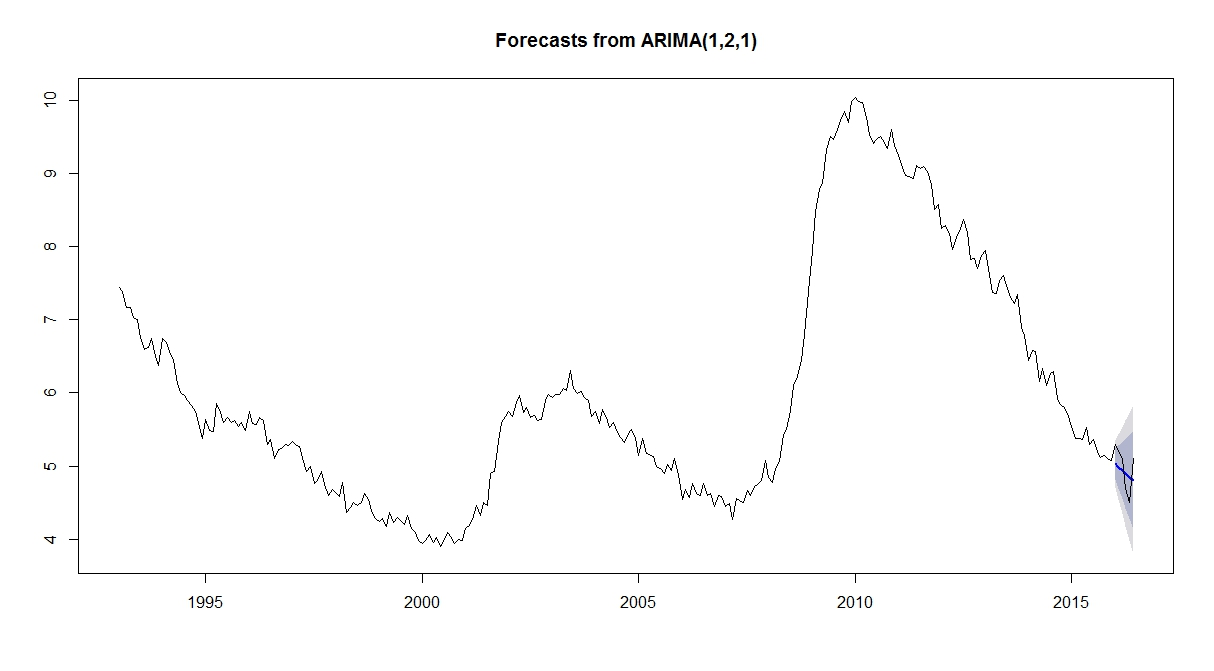
\includegraphics[width=\linewidth]{images/forejune}
 \end{figure}

I have built a few VAR models that we can use to compare against the currently favored ARIMA models. I have also cleaned up the \begin{verbatim}All_Final_Models.r\end{verbatim} script and removed all of the seasonally adjusted data and models. I will post about that next, but here is what I have found for the VAR model. First, i think it was very fun to play with the vars package. It has a lot of functionality and many different plots that can be called.

I ended up fitting 6 models in total. VAR(1), VAR(2), VAR(3) with no lags and then again with all of the ``xRegs'' lagged at various h (see Multivariate.r) for how i determined which lags to use. There is a lot of output that comes with each model so I am only going to post one so you get the idea. You should be able to run the VAR.r script without incident if the data folder is a sub directory of your current R work space.

I decided to run up to a VAR(3) so that I could try to eliminate as much residual variance as possible. Sometimes in the ACF residuals plots you can see significant values in lag 12 even though we are using seasonally adjusted data. You dont see this in the unemployment rate acf plots which is good since thats what we are most interested in. You could probably argue that VAR(1) is good enough if you only wanted to look at unemployment. 

  \begin{figure}[H]
    	\centering
     	\caption{with June 2016}
     	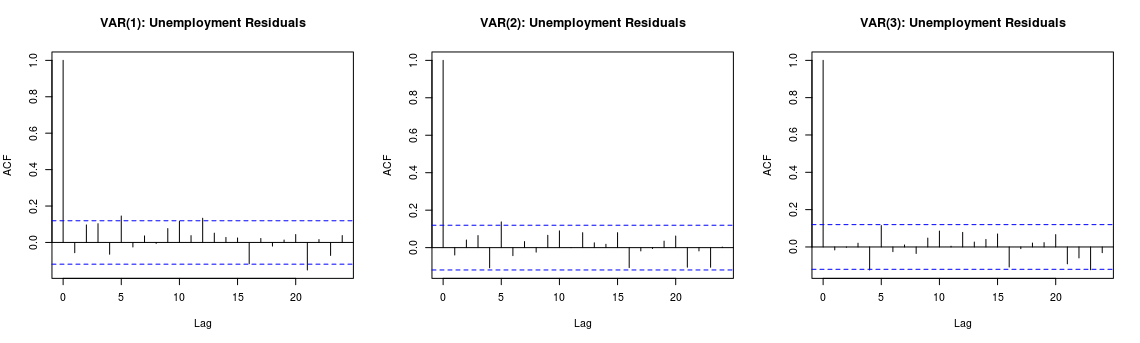
\includegraphics[width=\linewidth]{images/varUnemresid}
 \end{figure}
 
 Here is a plot of the unemployment series in the best performing model by AIC: Var(2) with lagged xregs.
 
   \begin{figure}[H]
    	\centering
     	\caption{fit and residuals}
     	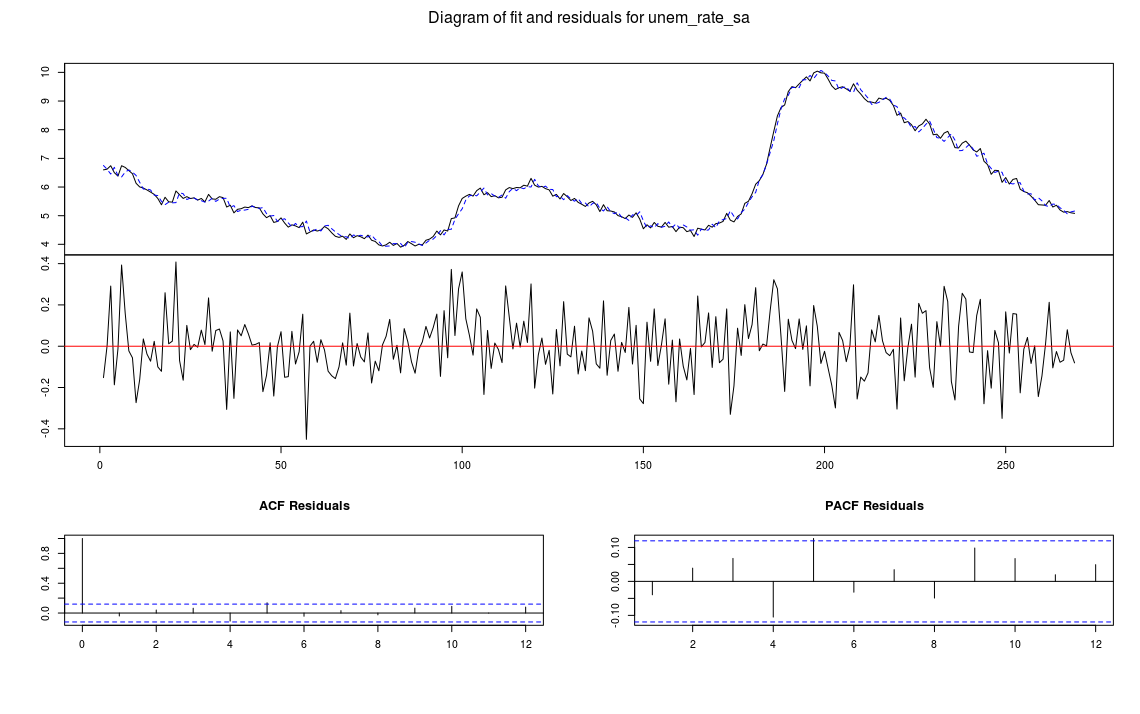
\includegraphics[width=\linewidth]{images/unem_rate_fit_resid}
 \end{figure}
 
 There is also forecasting functionality in the package which is nice because in the case of an ARIMA model with xregs, you dont have to forecast the xregs. Vars will do that for you since all of they are essentially AR(p) models that only use lagged values to forecast.
 
    \begin{figure}[H]
    	\centering
     	\caption{Var(2) Forcast 5 mo}
     	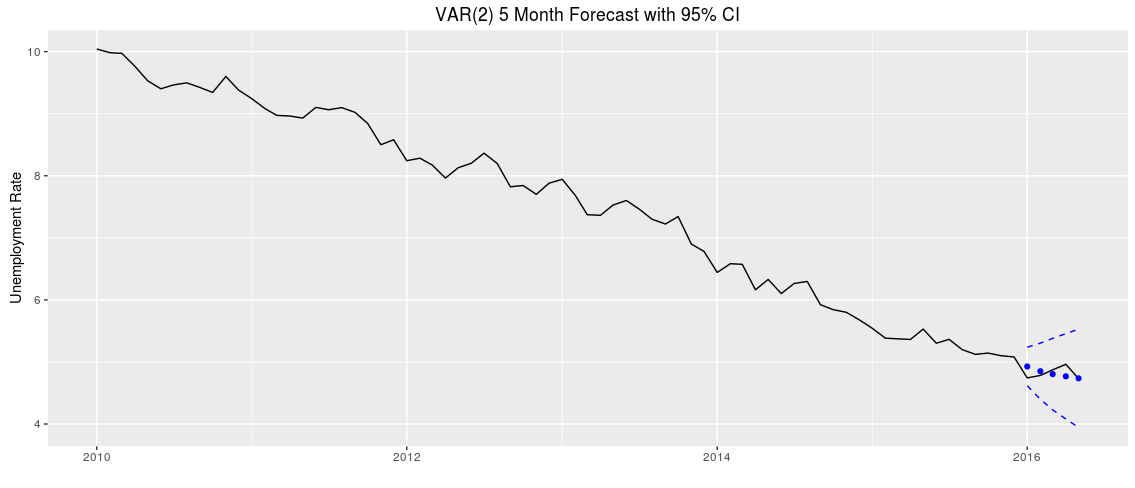
\includegraphics[width=\linewidth]{images/var25mo}
 \end{figure}
 
I also built a few VAR models. By VARselect, BIC suggests VAR(1) HQ suggest VAR(2). The VAR(1) results only show the \begin{verbatim}retail_sales_sa.l1 and recession_ind.l1\end{verbatim} besides \begin{verbatim}unem_rate_sa.l1\end{verbatim} were significant predictors. I checked the correlation among these predictors and found that variables \begin{verbatim}industrial_production, manufacturers_new_orders, \end{verbatim} \begin{verbatim}house_price_sa, construction_spend, and retail_sales\end{verbatim} are highly correlated.

    \begin{figure}[H]
    	\centering
     	\caption{Scatterplot matrix}
     	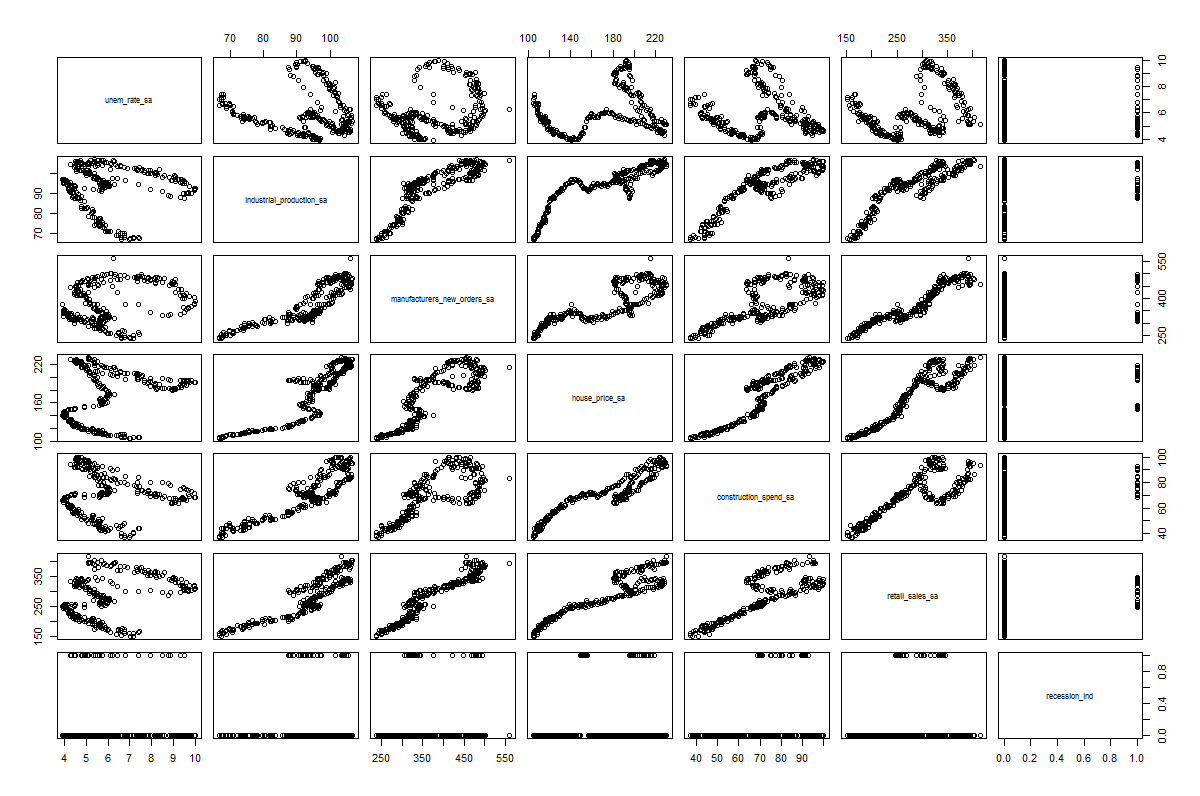
\includegraphics[width=\linewidth]{images/varcorrelation}
 \end{figure}

It might be reasonable to leave out some highly correlated variables. Thus, I then fitted two models with only \begin{verbatim}unem_rate, retail_sales, and recession_ind\end{verbatim}. Here are the AICs and BICs.

\begin{verbatim}
AIC(M1$varresult$unem_rate_sa) # -253.317
AIC(M2$varresult$unem_rate_sa) # -252.6457
AIC(M3$varresult$unem_rate_sa) # -247.1147
AIC(M4$varresult$unem_rate_sa) # -251.6351

BIC(M1$varresult$unem_rate_sa) # -217.1493
BIC(M2$varresult$unem_rate_sa) # -191.2225
BIC(M3$varresult$unem_rate_sa) # -225.414
BIC(M4$varresult$unem_rate_sa) # -219.117

AICs suggest the original VAR(1) model. 
The BICs suggest the VAR(1) with only three variables. 
\end{verbatim}

    \begin{figure}[H]
    	\centering
     	\caption{Plots of above}
     	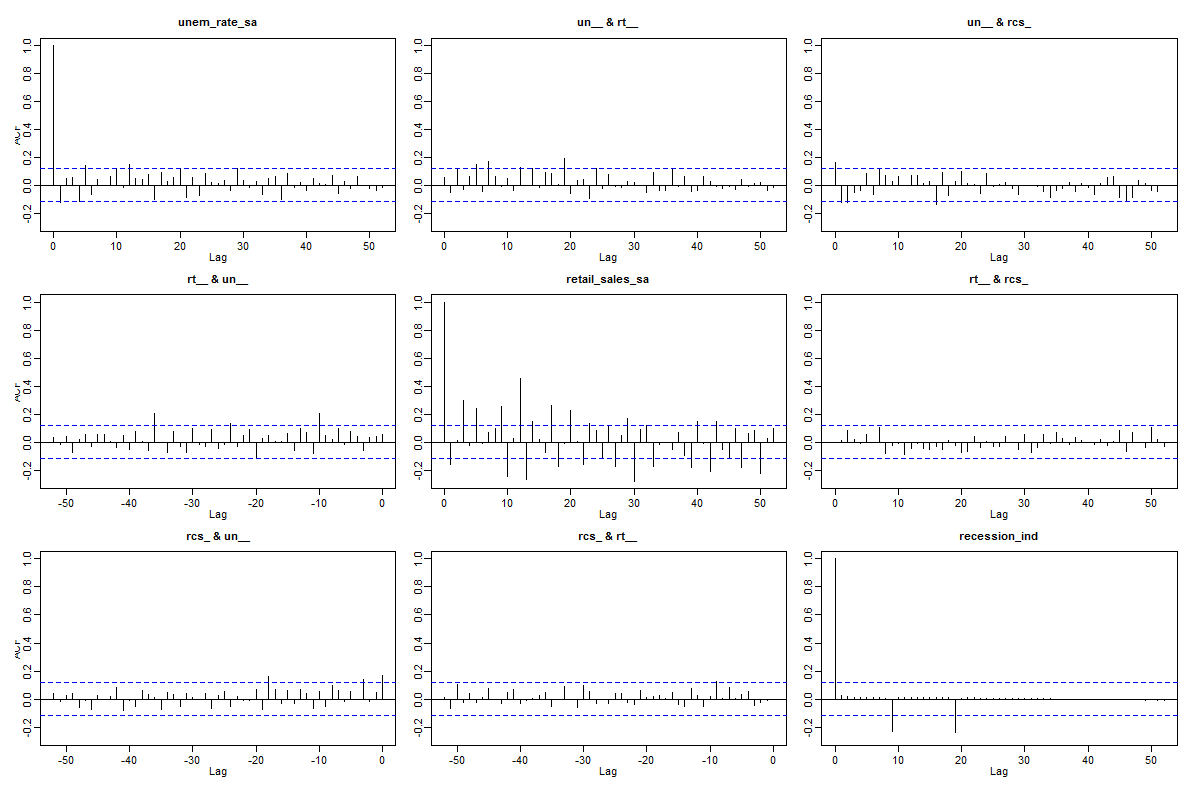
\includegraphics[width=\linewidth]{images/boplots}
 \end{figure}

Yeah, i am not sure how appropriate it is to include the recession indicator, but that is very interesting that it improved AIC that much. I will add it to my version as well since I am probably using different lags for all of the variables... we will see how it shakes out.. either way I will add what you have done to the \begin{verbatim}All_Final_Moels.r\end{verbatim} and then we can decide as a group which to mention in the write up. Im finalizing some tables right now that compares all of the best performing models everyone has submitted.. i will post the results for discussion shortly.

One point though that I read about... since VARs do not require data to be stationary maybe it is okay to include it... has anyone come across anything in the literature that might have looked at this?

Thanks! This issue might need some discussion. Btw, I actually prefer the model 3 among the set I proposed. It has the smallest BIC and really simple (two leading variables and 1 lag). I also saw some problems of the acf plots. I tried to fit stationary data by differencing. But that didn't help much and ruined model fitting in terms AIC and BIC. Any suggestions to further explore on this issue would be appreciated.

Okay, I have compiled all of the models we have considered into the AllFinalModels.r script... so far we have 2 model types ARIMA and VAR. I do not think we should actually talk about or show diagnostic plots on all of these models. Maybe just focus on the top 2 in the 3rd table, but I do think we should perhaps show tables of all of the models we considered.

\textit{These tables are included earlier.}

5 Month Forecasts for the 2 best Models

Since we decomposed and adjusted the seasonal data ourselves, it differs slightly from what you would see on the BLS website so I applied the same seasonal adjustment to the first 5 months of unemployment that came with the original data set. Overall the two plots are very similar.

It also looks like the VAR model produced a slightly better forecast over this period, however the confidence intervals of the models overlap substantially.

The forecasts start to look significantly different when you look at the longer term forecasts. This plot shows a 36 month forecast for the two best models. We can see how the confidence interval of the ARIMA model quickly explodes, perhaps indicating that it is not a good choice for long term forecasts.

\textit{All of the previously mentioned plots are already included earlier except for:}
    \begin{figure}[H]
    	\centering
     	\caption{Other plot}
     	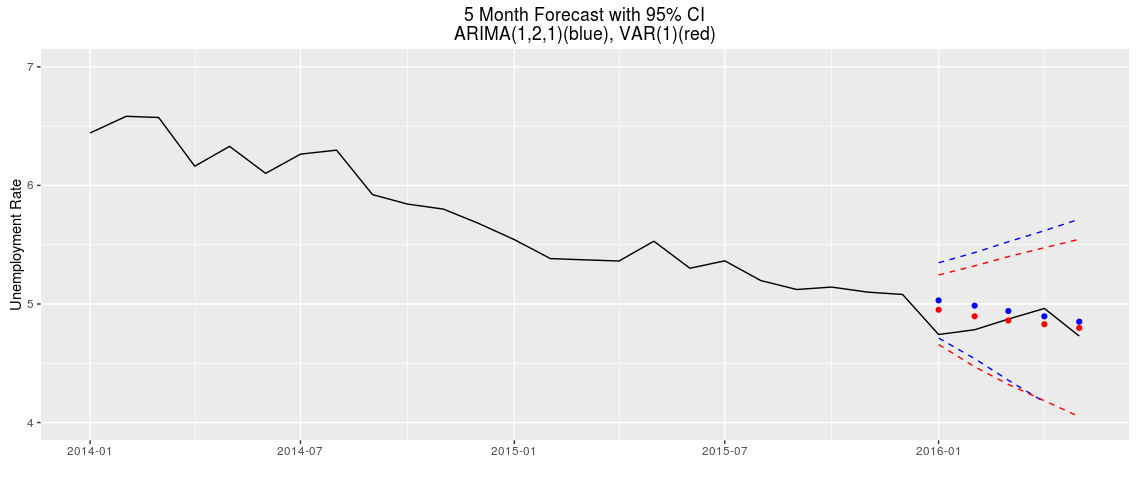
\includegraphics[width=\linewidth]{images/arimavarforcastalso}
 \end{figure}
 
 
 Note on best VAR
For the best VAR model shown in the 2nd table, all of the variables are present. The inclusion of the recession indicator significantly improves the overall fit as well as the look of the forecast plot. There are a few variables in the VAR model that do not measure as being significant. When taking those parameters out the longterm forecast looks a bit more aggressive. The AIC and BIC are both a couple points improved if you remove the insignificant variables though. I can strip them back out depending on what everyone thinks we should do. Here is a plot with the insignificant variables removed.

As far as model choice goes, i tend to favor the VAR rather than the ARIMA based on the model fit and forecast plots. The ARIMA(1,2,1) has 2 parameters, and the VAR(1) has 9 parameters (7 if we remove the insignificant variables). The inclusion of the recession indicator really helps the fit. So far I have not seen anything online that says its inappropriate to use an indicator variable in a VAR model.

Please everyone weigh in on the model selection. If we elect not to use recession indicator then on the second table, mdl.1 is the best BIC and model 5 is the best AIC. If we only use the significant variables then the mdl.1 VAR(1) becomes the best model with an AIC of -225 and BIC of -200 which is right there with the ARIMA(1,2,1) and it would have 6 parameters.

This is very nice. I like the recession indicator. I think it is consistent with the literature. It is a way of dealing with the fact that we would expect unemployment to increase more rapidly during a recession than at other times. From: (Montgomery et al., 1998) "Evidently the unemployment rate has a strong tendency to move countercyclically, upward in general business slowdowns and contractions and downward in speedups and expansions. ...univariate linear models are not able to accurately represent these asymmetric cycles. ...the contraction phases in the U.S. economy tend to be shorter than the expansion phases. It should also be noted that forecasting unemployment is much more difficult during periods when it is rapidly increasing than during more stable periods."



Here are the two equations without the insignificant variables. Im in favor of dropping out the insignificant variables even though it changes the long term forecast picture. If no one has a problem, im going to drop them in the code and rerun the tables (IndustrialProduction, ManufacturersNewOrders, HomePrices). Looks to me like the VAR(1) is the way to go.

\begin{verbatim}
VAR(1)
Unemployment = .935 + .0041 t + .975 
Unemployment_{t-1} + .004 ConstructionSpend_{t-1}
 - .005 RetailSales_{t-1} + .19 RecessionIndicator_{t-1}
 + w_t
AIC: -256, BIC: -231

ARIMA(1,2,1)
Unemployment = -.2021 
Unemployment_{t-1} - .8078 w_{t-1} + w_t
AIC: -212, BIC: -201
\end{verbatim}

Even though there are more parameters, VAR(1) does seem the best. It incorporates some of our original ideas and beats everything else in AIC. On the other hand, RetailSales and ConstructionSpend have small coefficients; do they really add much to the model?

Yeah. Keep in mind they are in different scales.

I the VAR(1) is good, too. For our final discussion, do we want to just focus on one model, or were we going to discuss both. I think it might be easier just to stick with one.

I think we want to present one model ultimately, but I also think that part of the process is how we went about selecting the model we chose. Maybe mention it more in the write up than the final presentation. I dont know.



The VAR models in the literature have been outperforming the ARIMA models significantly. Although some of the more recent articles are using VAR to model different predictors I still think it is good justification. For example:

(Barnichon \& Garda, 2016)
"Finally, the large improvements in forecasting performances were obtained with simple VAR-based forecasts of the worker flows. "

(Meyer \& Tasci, 2015)
"So far our results indicate that the VAR model delivers the most accurate forecasts for up to 2 quarters ahead, and the FLOW-UC model presents the most potential for the farther
horizons,"

Updated the VAR to not include the insignificant variables I mentioned. The plots in \(All_Final_Models.r\) will reflect this... here are the updated tables now that those variables have been dropped. This matches the VAR equation i posted yesterday.

The professor seems to like the idea of splitting the data into training and validation sets. We didn't split the data but luckily we have the new 5 months data as a validation set. From looking at the plots, it seems hard to distinguish the performance of two models. I computed the mean squared error of forecasting of the two best models. 0.01505823 for ARIMA(1,2,1) and 0.009663836 for VAR(1). This quantitative measure also supports this VAR(1) model. Hope this would help a bit when we are comparing the two models. 
 
%----------------------------------------------------------------------------------------

\end{document}
